
% Default to the notebook output style

    


% Inherit from the specified cell style.




    
\documentclass[11pt]{article}

    
    
    \usepackage[T1]{fontenc}
    % Nicer default font (+ math font) than Computer Modern for most use cases
    \usepackage{mathpazo}

    % Basic figure setup, for now with no caption control since it's done
    % automatically by Pandoc (which extracts ![](path) syntax from Markdown).
    \usepackage{graphicx}
    % We will generate all images so they have a width \maxwidth. This means
    % that they will get their normal width if they fit onto the page, but
    % are scaled down if they would overflow the margins.
    \makeatletter
    \def\maxwidth{\ifdim\Gin@nat@width>\linewidth\linewidth
    \else\Gin@nat@width\fi}
    \makeatother
    \let\Oldincludegraphics\includegraphics
    % Set max figure width to be 80% of text width, for now hardcoded.
    \renewcommand{\includegraphics}[1]{\Oldincludegraphics[width=.8\maxwidth]{#1}}
    % Ensure that by default, figures have no caption (until we provide a
    % proper Figure object with a Caption API and a way to capture that
    % in the conversion process - todo).
    \usepackage{caption}
    \DeclareCaptionLabelFormat{nolabel}{}
    \captionsetup{labelformat=nolabel}

    \usepackage{adjustbox} % Used to constrain images to a maximum size 
    \usepackage{xcolor} % Allow colors to be defined
    \usepackage{enumerate} % Needed for markdown enumerations to work
    \usepackage{geometry} % Used to adjust the document margins
    \usepackage{amsmath} % Equations
    \usepackage{amssymb} % Equations
    \usepackage{textcomp} % defines textquotesingle
    % Hack from http://tex.stackexchange.com/a/47451/13684:
    \AtBeginDocument{%
        \def\PYZsq{\textquotesingle}% Upright quotes in Pygmentized code
    }
    \usepackage{upquote} % Upright quotes for verbatim code
    \usepackage{eurosym} % defines \euro
    \usepackage[mathletters]{ucs} % Extended unicode (utf-8) support
    \usepackage[utf8x]{inputenc} % Allow utf-8 characters in the tex document
    \usepackage{fancyvrb} % verbatim replacement that allows latex
    \usepackage{grffile} % extends the file name processing of package graphics 
                         % to support a larger range 
    % The hyperref package gives us a pdf with properly built
    % internal navigation ('pdf bookmarks' for the table of contents,
    % internal cross-reference links, web links for URLs, etc.)
    \usepackage{hyperref}
    \usepackage{longtable} % longtable support required by pandoc >1.10
    \usepackage{booktabs}  % table support for pandoc > 1.12.2
    \usepackage[inline]{enumitem} % IRkernel/repr support (it uses the enumerate* environment)
    \usepackage[normalem]{ulem} % ulem is needed to support strikethroughs (\sout)
                                % normalem makes italics be italics, not underlines
    

    
    
    % Colors for the hyperref package
    \definecolor{urlcolor}{rgb}{0,.145,.698}
    \definecolor{linkcolor}{rgb}{.71,0.21,0.01}
    \definecolor{citecolor}{rgb}{.12,.54,.11}

    % ANSI colors
    \definecolor{ansi-black}{HTML}{3E424D}
    \definecolor{ansi-black-intense}{HTML}{282C36}
    \definecolor{ansi-red}{HTML}{E75C58}
    \definecolor{ansi-red-intense}{HTML}{B22B31}
    \definecolor{ansi-green}{HTML}{00A250}
    \definecolor{ansi-green-intense}{HTML}{007427}
    \definecolor{ansi-yellow}{HTML}{DDB62B}
    \definecolor{ansi-yellow-intense}{HTML}{B27D12}
    \definecolor{ansi-blue}{HTML}{208FFB}
    \definecolor{ansi-blue-intense}{HTML}{0065CA}
    \definecolor{ansi-magenta}{HTML}{D160C4}
    \definecolor{ansi-magenta-intense}{HTML}{A03196}
    \definecolor{ansi-cyan}{HTML}{60C6C8}
    \definecolor{ansi-cyan-intense}{HTML}{258F8F}
    \definecolor{ansi-white}{HTML}{C5C1B4}
    \definecolor{ansi-white-intense}{HTML}{A1A6B2}

    % commands and environments needed by pandoc snippets
    % extracted from the output of `pandoc -s`
    \providecommand{\tightlist}{%
      \setlength{\itemsep}{0pt}\setlength{\parskip}{0pt}}
    \DefineVerbatimEnvironment{Highlighting}{Verbatim}{commandchars=\\\{\}}
    % Add ',fontsize=\small' for more characters per line
    \newenvironment{Shaded}{}{}
    \newcommand{\KeywordTok}[1]{\textcolor[rgb]{0.00,0.44,0.13}{\textbf{{#1}}}}
    \newcommand{\DataTypeTok}[1]{\textcolor[rgb]{0.56,0.13,0.00}{{#1}}}
    \newcommand{\DecValTok}[1]{\textcolor[rgb]{0.25,0.63,0.44}{{#1}}}
    \newcommand{\BaseNTok}[1]{\textcolor[rgb]{0.25,0.63,0.44}{{#1}}}
    \newcommand{\FloatTok}[1]{\textcolor[rgb]{0.25,0.63,0.44}{{#1}}}
    \newcommand{\CharTok}[1]{\textcolor[rgb]{0.25,0.44,0.63}{{#1}}}
    \newcommand{\StringTok}[1]{\textcolor[rgb]{0.25,0.44,0.63}{{#1}}}
    \newcommand{\CommentTok}[1]{\textcolor[rgb]{0.38,0.63,0.69}{\textit{{#1}}}}
    \newcommand{\OtherTok}[1]{\textcolor[rgb]{0.00,0.44,0.13}{{#1}}}
    \newcommand{\AlertTok}[1]{\textcolor[rgb]{1.00,0.00,0.00}{\textbf{{#1}}}}
    \newcommand{\FunctionTok}[1]{\textcolor[rgb]{0.02,0.16,0.49}{{#1}}}
    \newcommand{\RegionMarkerTok}[1]{{#1}}
    \newcommand{\ErrorTok}[1]{\textcolor[rgb]{1.00,0.00,0.00}{\textbf{{#1}}}}
    \newcommand{\NormalTok}[1]{{#1}}
    
    % Additional commands for more recent versions of Pandoc
    \newcommand{\ConstantTok}[1]{\textcolor[rgb]{0.53,0.00,0.00}{{#1}}}
    \newcommand{\SpecialCharTok}[1]{\textcolor[rgb]{0.25,0.44,0.63}{{#1}}}
    \newcommand{\VerbatimStringTok}[1]{\textcolor[rgb]{0.25,0.44,0.63}{{#1}}}
    \newcommand{\SpecialStringTok}[1]{\textcolor[rgb]{0.73,0.40,0.53}{{#1}}}
    \newcommand{\ImportTok}[1]{{#1}}
    \newcommand{\DocumentationTok}[1]{\textcolor[rgb]{0.73,0.13,0.13}{\textit{{#1}}}}
    \newcommand{\AnnotationTok}[1]{\textcolor[rgb]{0.38,0.63,0.69}{\textbf{\textit{{#1}}}}}
    \newcommand{\CommentVarTok}[1]{\textcolor[rgb]{0.38,0.63,0.69}{\textbf{\textit{{#1}}}}}
    \newcommand{\VariableTok}[1]{\textcolor[rgb]{0.10,0.09,0.49}{{#1}}}
    \newcommand{\ControlFlowTok}[1]{\textcolor[rgb]{0.00,0.44,0.13}{\textbf{{#1}}}}
    \newcommand{\OperatorTok}[1]{\textcolor[rgb]{0.40,0.40,0.40}{{#1}}}
    \newcommand{\BuiltInTok}[1]{{#1}}
    \newcommand{\ExtensionTok}[1]{{#1}}
    \newcommand{\PreprocessorTok}[1]{\textcolor[rgb]{0.74,0.48,0.00}{{#1}}}
    \newcommand{\AttributeTok}[1]{\textcolor[rgb]{0.49,0.56,0.16}{{#1}}}
    \newcommand{\InformationTok}[1]{\textcolor[rgb]{0.38,0.63,0.69}{\textbf{\textit{{#1}}}}}
    \newcommand{\WarningTok}[1]{\textcolor[rgb]{0.38,0.63,0.69}{\textbf{\textit{{#1}}}}}
    
    
    % Define a nice break command that doesn't care if a line doesn't already
    % exist.
    \def\br{\hspace*{\fill} \\* }
    % Math Jax compatability definitions
    \def\gt{>}
    \def\lt{<}
    % Document parameters
    \title{linear\_regression}
    
    
    

    % Pygments definitions
    
\makeatletter
\def\PY@reset{\let\PY@it=\relax \let\PY@bf=\relax%
    \let\PY@ul=\relax \let\PY@tc=\relax%
    \let\PY@bc=\relax \let\PY@ff=\relax}
\def\PY@tok#1{\csname PY@tok@#1\endcsname}
\def\PY@toks#1+{\ifx\relax#1\empty\else%
    \PY@tok{#1}\expandafter\PY@toks\fi}
\def\PY@do#1{\PY@bc{\PY@tc{\PY@ul{%
    \PY@it{\PY@bf{\PY@ff{#1}}}}}}}
\def\PY#1#2{\PY@reset\PY@toks#1+\relax+\PY@do{#2}}

\expandafter\def\csname PY@tok@gd\endcsname{\def\PY@tc##1{\textcolor[rgb]{0.63,0.00,0.00}{##1}}}
\expandafter\def\csname PY@tok@gu\endcsname{\let\PY@bf=\textbf\def\PY@tc##1{\textcolor[rgb]{0.50,0.00,0.50}{##1}}}
\expandafter\def\csname PY@tok@gt\endcsname{\def\PY@tc##1{\textcolor[rgb]{0.00,0.27,0.87}{##1}}}
\expandafter\def\csname PY@tok@gs\endcsname{\let\PY@bf=\textbf}
\expandafter\def\csname PY@tok@gr\endcsname{\def\PY@tc##1{\textcolor[rgb]{1.00,0.00,0.00}{##1}}}
\expandafter\def\csname PY@tok@cm\endcsname{\let\PY@it=\textit\def\PY@tc##1{\textcolor[rgb]{0.25,0.50,0.50}{##1}}}
\expandafter\def\csname PY@tok@vg\endcsname{\def\PY@tc##1{\textcolor[rgb]{0.10,0.09,0.49}{##1}}}
\expandafter\def\csname PY@tok@vi\endcsname{\def\PY@tc##1{\textcolor[rgb]{0.10,0.09,0.49}{##1}}}
\expandafter\def\csname PY@tok@vm\endcsname{\def\PY@tc##1{\textcolor[rgb]{0.10,0.09,0.49}{##1}}}
\expandafter\def\csname PY@tok@mh\endcsname{\def\PY@tc##1{\textcolor[rgb]{0.40,0.40,0.40}{##1}}}
\expandafter\def\csname PY@tok@cs\endcsname{\let\PY@it=\textit\def\PY@tc##1{\textcolor[rgb]{0.25,0.50,0.50}{##1}}}
\expandafter\def\csname PY@tok@ge\endcsname{\let\PY@it=\textit}
\expandafter\def\csname PY@tok@vc\endcsname{\def\PY@tc##1{\textcolor[rgb]{0.10,0.09,0.49}{##1}}}
\expandafter\def\csname PY@tok@il\endcsname{\def\PY@tc##1{\textcolor[rgb]{0.40,0.40,0.40}{##1}}}
\expandafter\def\csname PY@tok@go\endcsname{\def\PY@tc##1{\textcolor[rgb]{0.53,0.53,0.53}{##1}}}
\expandafter\def\csname PY@tok@cp\endcsname{\def\PY@tc##1{\textcolor[rgb]{0.74,0.48,0.00}{##1}}}
\expandafter\def\csname PY@tok@gi\endcsname{\def\PY@tc##1{\textcolor[rgb]{0.00,0.63,0.00}{##1}}}
\expandafter\def\csname PY@tok@gh\endcsname{\let\PY@bf=\textbf\def\PY@tc##1{\textcolor[rgb]{0.00,0.00,0.50}{##1}}}
\expandafter\def\csname PY@tok@ni\endcsname{\let\PY@bf=\textbf\def\PY@tc##1{\textcolor[rgb]{0.60,0.60,0.60}{##1}}}
\expandafter\def\csname PY@tok@nl\endcsname{\def\PY@tc##1{\textcolor[rgb]{0.63,0.63,0.00}{##1}}}
\expandafter\def\csname PY@tok@nn\endcsname{\let\PY@bf=\textbf\def\PY@tc##1{\textcolor[rgb]{0.00,0.00,1.00}{##1}}}
\expandafter\def\csname PY@tok@no\endcsname{\def\PY@tc##1{\textcolor[rgb]{0.53,0.00,0.00}{##1}}}
\expandafter\def\csname PY@tok@na\endcsname{\def\PY@tc##1{\textcolor[rgb]{0.49,0.56,0.16}{##1}}}
\expandafter\def\csname PY@tok@nb\endcsname{\def\PY@tc##1{\textcolor[rgb]{0.00,0.50,0.00}{##1}}}
\expandafter\def\csname PY@tok@nc\endcsname{\let\PY@bf=\textbf\def\PY@tc##1{\textcolor[rgb]{0.00,0.00,1.00}{##1}}}
\expandafter\def\csname PY@tok@nd\endcsname{\def\PY@tc##1{\textcolor[rgb]{0.67,0.13,1.00}{##1}}}
\expandafter\def\csname PY@tok@ne\endcsname{\let\PY@bf=\textbf\def\PY@tc##1{\textcolor[rgb]{0.82,0.25,0.23}{##1}}}
\expandafter\def\csname PY@tok@nf\endcsname{\def\PY@tc##1{\textcolor[rgb]{0.00,0.00,1.00}{##1}}}
\expandafter\def\csname PY@tok@si\endcsname{\let\PY@bf=\textbf\def\PY@tc##1{\textcolor[rgb]{0.73,0.40,0.53}{##1}}}
\expandafter\def\csname PY@tok@s2\endcsname{\def\PY@tc##1{\textcolor[rgb]{0.73,0.13,0.13}{##1}}}
\expandafter\def\csname PY@tok@nt\endcsname{\let\PY@bf=\textbf\def\PY@tc##1{\textcolor[rgb]{0.00,0.50,0.00}{##1}}}
\expandafter\def\csname PY@tok@nv\endcsname{\def\PY@tc##1{\textcolor[rgb]{0.10,0.09,0.49}{##1}}}
\expandafter\def\csname PY@tok@s1\endcsname{\def\PY@tc##1{\textcolor[rgb]{0.73,0.13,0.13}{##1}}}
\expandafter\def\csname PY@tok@dl\endcsname{\def\PY@tc##1{\textcolor[rgb]{0.73,0.13,0.13}{##1}}}
\expandafter\def\csname PY@tok@ch\endcsname{\let\PY@it=\textit\def\PY@tc##1{\textcolor[rgb]{0.25,0.50,0.50}{##1}}}
\expandafter\def\csname PY@tok@m\endcsname{\def\PY@tc##1{\textcolor[rgb]{0.40,0.40,0.40}{##1}}}
\expandafter\def\csname PY@tok@gp\endcsname{\let\PY@bf=\textbf\def\PY@tc##1{\textcolor[rgb]{0.00,0.00,0.50}{##1}}}
\expandafter\def\csname PY@tok@sh\endcsname{\def\PY@tc##1{\textcolor[rgb]{0.73,0.13,0.13}{##1}}}
\expandafter\def\csname PY@tok@ow\endcsname{\let\PY@bf=\textbf\def\PY@tc##1{\textcolor[rgb]{0.67,0.13,1.00}{##1}}}
\expandafter\def\csname PY@tok@sx\endcsname{\def\PY@tc##1{\textcolor[rgb]{0.00,0.50,0.00}{##1}}}
\expandafter\def\csname PY@tok@bp\endcsname{\def\PY@tc##1{\textcolor[rgb]{0.00,0.50,0.00}{##1}}}
\expandafter\def\csname PY@tok@c1\endcsname{\let\PY@it=\textit\def\PY@tc##1{\textcolor[rgb]{0.25,0.50,0.50}{##1}}}
\expandafter\def\csname PY@tok@fm\endcsname{\def\PY@tc##1{\textcolor[rgb]{0.00,0.00,1.00}{##1}}}
\expandafter\def\csname PY@tok@o\endcsname{\def\PY@tc##1{\textcolor[rgb]{0.40,0.40,0.40}{##1}}}
\expandafter\def\csname PY@tok@kc\endcsname{\let\PY@bf=\textbf\def\PY@tc##1{\textcolor[rgb]{0.00,0.50,0.00}{##1}}}
\expandafter\def\csname PY@tok@c\endcsname{\let\PY@it=\textit\def\PY@tc##1{\textcolor[rgb]{0.25,0.50,0.50}{##1}}}
\expandafter\def\csname PY@tok@mf\endcsname{\def\PY@tc##1{\textcolor[rgb]{0.40,0.40,0.40}{##1}}}
\expandafter\def\csname PY@tok@err\endcsname{\def\PY@bc##1{\setlength{\fboxsep}{0pt}\fcolorbox[rgb]{1.00,0.00,0.00}{1,1,1}{\strut ##1}}}
\expandafter\def\csname PY@tok@mb\endcsname{\def\PY@tc##1{\textcolor[rgb]{0.40,0.40,0.40}{##1}}}
\expandafter\def\csname PY@tok@ss\endcsname{\def\PY@tc##1{\textcolor[rgb]{0.10,0.09,0.49}{##1}}}
\expandafter\def\csname PY@tok@sr\endcsname{\def\PY@tc##1{\textcolor[rgb]{0.73,0.40,0.53}{##1}}}
\expandafter\def\csname PY@tok@mo\endcsname{\def\PY@tc##1{\textcolor[rgb]{0.40,0.40,0.40}{##1}}}
\expandafter\def\csname PY@tok@kd\endcsname{\let\PY@bf=\textbf\def\PY@tc##1{\textcolor[rgb]{0.00,0.50,0.00}{##1}}}
\expandafter\def\csname PY@tok@mi\endcsname{\def\PY@tc##1{\textcolor[rgb]{0.40,0.40,0.40}{##1}}}
\expandafter\def\csname PY@tok@kn\endcsname{\let\PY@bf=\textbf\def\PY@tc##1{\textcolor[rgb]{0.00,0.50,0.00}{##1}}}
\expandafter\def\csname PY@tok@cpf\endcsname{\let\PY@it=\textit\def\PY@tc##1{\textcolor[rgb]{0.25,0.50,0.50}{##1}}}
\expandafter\def\csname PY@tok@kr\endcsname{\let\PY@bf=\textbf\def\PY@tc##1{\textcolor[rgb]{0.00,0.50,0.00}{##1}}}
\expandafter\def\csname PY@tok@s\endcsname{\def\PY@tc##1{\textcolor[rgb]{0.73,0.13,0.13}{##1}}}
\expandafter\def\csname PY@tok@kp\endcsname{\def\PY@tc##1{\textcolor[rgb]{0.00,0.50,0.00}{##1}}}
\expandafter\def\csname PY@tok@w\endcsname{\def\PY@tc##1{\textcolor[rgb]{0.73,0.73,0.73}{##1}}}
\expandafter\def\csname PY@tok@kt\endcsname{\def\PY@tc##1{\textcolor[rgb]{0.69,0.00,0.25}{##1}}}
\expandafter\def\csname PY@tok@sc\endcsname{\def\PY@tc##1{\textcolor[rgb]{0.73,0.13,0.13}{##1}}}
\expandafter\def\csname PY@tok@sb\endcsname{\def\PY@tc##1{\textcolor[rgb]{0.73,0.13,0.13}{##1}}}
\expandafter\def\csname PY@tok@sa\endcsname{\def\PY@tc##1{\textcolor[rgb]{0.73,0.13,0.13}{##1}}}
\expandafter\def\csname PY@tok@k\endcsname{\let\PY@bf=\textbf\def\PY@tc##1{\textcolor[rgb]{0.00,0.50,0.00}{##1}}}
\expandafter\def\csname PY@tok@se\endcsname{\let\PY@bf=\textbf\def\PY@tc##1{\textcolor[rgb]{0.73,0.40,0.13}{##1}}}
\expandafter\def\csname PY@tok@sd\endcsname{\let\PY@it=\textit\def\PY@tc##1{\textcolor[rgb]{0.73,0.13,0.13}{##1}}}

\def\PYZbs{\char`\\}
\def\PYZus{\char`\_}
\def\PYZob{\char`\{}
\def\PYZcb{\char`\}}
\def\PYZca{\char`\^}
\def\PYZam{\char`\&}
\def\PYZlt{\char`\<}
\def\PYZgt{\char`\>}
\def\PYZsh{\char`\#}
\def\PYZpc{\char`\%}
\def\PYZdl{\char`\$}
\def\PYZhy{\char`\-}
\def\PYZsq{\char`\'}
\def\PYZdq{\char`\"}
\def\PYZti{\char`\~}
% for compatibility with earlier versions
\def\PYZat{@}
\def\PYZlb{[}
\def\PYZrb{]}
\makeatother


    % Exact colors from NB
    \definecolor{incolor}{rgb}{0.0, 0.0, 0.5}
    \definecolor{outcolor}{rgb}{0.545, 0.0, 0.0}



    
    % Prevent overflowing lines due to hard-to-break entities
    \sloppy 
    % Setup hyperref package
    \hypersetup{
      breaklinks=true,  % so long urls are correctly broken across lines
      colorlinks=true,
      urlcolor=urlcolor,
      linkcolor=linkcolor,
      citecolor=citecolor,
      }
    % Slightly bigger margins than the latex defaults
    
    \geometry{verbose,tmargin=1in,bmargin=1in,lmargin=1in,rmargin=1in}
    
    

    \begin{document}
    
    
    \maketitle
    
    

    
    \section{Linear Regression}\label{linear-regression}

\emph{Authors: Kevin Markham (Washington, D.C.), Ed Podojil (New York
City)}

    \paragraph{Learning Objectives}\label{learning-objectives}

\begin{itemize}
\tightlist
\item
  Define data modeling and simple linear regression.
\item
  Build a linear regression model using a data set that meets the
  linearity assumption using the scikit-learn library.
\item
  Understand and identify multicollinearity in a multiple regression.
\end{itemize}

    \subsubsection{Lesson Guide}\label{lesson-guide}

\begin{itemize}
\tightlist
\item
  Section \ref{introduce-the-bikeshare-dataset}

  \begin{itemize}
  \tightlist
  \item
    Section \ref{read-in-the--capital-bikeshare-data}
  \item
    Section \ref{visualizing-the-data}
  \end{itemize}
\item
  Section \ref{linear-regression-basics}

  \begin{itemize}
  \tightlist
  \item
    Section \ref{form-of-linear-regression}
  \end{itemize}
\item
  Section \ref{overview-of-supervised-learning}

  \begin{itemize}
  \tightlist
  \item
    Section \ref{benefits-and-drawbacks-of-scikit-learn}
  \item
    Section \ref{requirements-for-working-with-data-in-scikit-learn}
  \item
    Section \ref{building-a-linear-regression-model-in-sklearn}
  \item
    Section \ref{scikit-learns--step-modeling-pattern}
  \end{itemize}
\item
  Section \ref{build-a-linear-regression-model}
\item
  Section \ref{using-the-model-for-prediction}

  \begin{itemize}
  \tightlist
  \item
    Section \ref{does-the-scale-of-the-features-matter}
  \end{itemize}
\item
  Section \ref{work-with-multiple-features}

  \begin{itemize}
  \tightlist
  \item
    Section \ref{visualizing-the-data-part-}
  \item
    Section \ref{adding-more-features-to-the-model}
  \end{itemize}
\item
  Section \ref{what-is-multicollinearity}
\item
  Section \ref{how-to-select-a-model}

  \begin{itemize}
  \tightlist
  \item
    Section \ref{feature-selection}
  \item
    Section \ref{evaluation-metrics-for-regression-problems}
  \item
    Section \ref{comparing-models-with-traintest-split-and-rmse}
  \item
    Section \ref{comparing-testing-rmse-with-null-rmse}
  \end{itemize}
\item
  Section \ref{feature-engineering-to-improve-performance}

  \begin{itemize}
  \tightlist
  \item
    Section \ref{handling-categorical-features}
  \item
    Section \ref{feature-engineering}
  \end{itemize}
\item
  Section \ref{bonus-material-regularization}

  \begin{itemize}
  \tightlist
  \item
    Section \ref{how-does-regularization-work}
  \item
    Section \ref{lasso-and-ridge-path-diagrams}
  \item
    Section \ref{advice-for-applying-regularization}
  \item
    Section \ref{ridge-regression}
  \end{itemize}
\item
  Section \ref{comparing-linear-regression-with-other-models}
\end{itemize}

     \#\# Introduce the Bikeshare Data Set -\/-\/-

    We'll be working with a data set from Capital Bikeshare that was used in
a Kaggle competition
(\href{https://www.kaggle.com/c/bike-sharing-demand/data}{data
dictionary}).

The objective of the competition is to predict total ridership of
Capital Bikeshare in any given hour.

Demand forecasting is a common data science application. If we can
predict the quantity of demand, total ridership in a given hour, we can
create analytical tools to improve the bikeshare system. Some
applications would be: * Find where to site new bikeshare stations and
know how large of a station to build. * Calculate the expected wear and
tear on bikes and what the replacement costs will be. * Use a slightly
different research design to forecast full and empty stations and send a
service vehicle to "rebalance" the bikes from one station to another, as
sometimes bikeshare stations have no bikes or are completely full and
prevent use of the station.

Businesses aren't new to demand forecasting, but older methods suffered
from poor predictions at atypical small locations. Modern approaches
incorporate clusters and online data from Twitter and Google Trends to
improve prediction in these small locations.

    \begin{Verbatim}[commandchars=\\\{\}]
{\color{incolor}In [{\color{incolor}1}]:} \PY{k+kn}{import} \PY{n+nn}{pandas} \PY{k}{as} \PY{n+nn}{pd}
        \PY{k+kn}{import} \PY{n+nn}{numpy} \PY{k}{as} \PY{n+nn}{np}
        \PY{k+kn}{import} \PY{n+nn}{seaborn} \PY{k}{as} \PY{n+nn}{sns}
        \PY{k+kn}{import} \PY{n+nn}{matplotlib}\PY{n+nn}{.}\PY{n+nn}{pyplot} \PY{k}{as} \PY{n+nn}{plt}
        \PY{o}{\PYZpc{}}\PY{k}{matplotlib} inline
        \PY{o}{\PYZpc{}}\PY{k}{config} InlineBackend.figure\PYZus{}format = \PYZdq{}retina\PYZdq{}
        \PY{n}{plt}\PY{o}{.}\PY{n}{rcParams}\PY{p}{[}\PY{l+s+s1}{\PYZsq{}}\PY{l+s+s1}{figure.figsize}\PY{l+s+s1}{\PYZsq{}}\PY{p}{]} \PY{o}{=} \PY{p}{(}\PY{l+m+mi}{8}\PY{p}{,} \PY{l+m+mi}{6}\PY{p}{)}
        \PY{n}{plt}\PY{o}{.}\PY{n}{rcParams}\PY{p}{[}\PY{l+s+s1}{\PYZsq{}}\PY{l+s+s1}{font.size}\PY{l+s+s1}{\PYZsq{}}\PY{p}{]} \PY{o}{=} \PY{l+m+mi}{14}
        \PY{n}{plt}\PY{o}{.}\PY{n}{style}\PY{o}{.}\PY{n}{use}\PY{p}{(}\PY{l+s+s2}{\PYZdq{}}\PY{l+s+s2}{fivethirtyeight}\PY{l+s+s2}{\PYZdq{}}\PY{p}{)}
\end{Verbatim}


     \#\#\# Read In the Capital Bikeshare Data

    \begin{Verbatim}[commandchars=\\\{\}]
{\color{incolor}In [{\color{incolor}2}]:} \PY{c+c1}{\PYZsh{} Read the data and set the datetime as the index.}
        \PY{n}{url} \PY{o}{=} \PY{l+s+s1}{\PYZsq{}}\PY{l+s+s1}{./data/bikeshare.csv}\PY{l+s+s1}{\PYZsq{}}
        \PY{n}{bikes} \PY{o}{=} \PY{n}{pd}\PY{o}{.}\PY{n}{read\PYZus{}csv}\PY{p}{(}\PY{n}{url}\PY{p}{,} \PY{n}{index\PYZus{}col}\PY{o}{=}\PY{l+s+s1}{\PYZsq{}}\PY{l+s+s1}{datetime}\PY{l+s+s1}{\PYZsq{}}\PY{p}{,} 
                            \PY{n}{parse\PYZus{}dates}\PY{o}{=}\PY{k+kc}{True}\PY{p}{)}
\end{Verbatim}


    Notice that we used \texttt{index\_col} to set an index or primary key
for our data. In this case, the index of each row will be set to the
value of its \texttt{datetime} field.

We also ask Pandas to parse dates (if \texttt{parse\_dates=True}, for
the index only). So, rather than reading in a string, Pandas converts
the index string to a \texttt{datetime} object.

    \begin{Verbatim}[commandchars=\\\{\}]
{\color{incolor}In [{\color{incolor}3}]:} \PY{c+c1}{\PYZsh{} Preview the first five rows of the DataFrame.}
        \PY{n}{bikes}\PY{o}{.}\PY{n}{head}\PY{p}{(}\PY{p}{)}
\end{Verbatim}


\begin{Verbatim}[commandchars=\\\{\}]
{\color{outcolor}Out[{\color{outcolor}3}]:}                      season  holiday  workingday  weather  temp   atemp  \textbackslash{}
        datetime                                                                  
        2011-01-01 00:00:00       1        0           0        1  9.84  14.395   
        2011-01-01 01:00:00       1        0           0        1  9.02  13.635   
        2011-01-01 02:00:00       1        0           0        1  9.02  13.635   
        2011-01-01 03:00:00       1        0           0        1  9.84  14.395   
        2011-01-01 04:00:00       1        0           0        1  9.84  14.395   
        
                             humidity  windspeed  casual  registered  count  
        datetime                                                             
        2011-01-01 00:00:00        81        0.0       3          13     16  
        2011-01-01 01:00:00        80        0.0       8          32     40  
        2011-01-01 02:00:00        80        0.0       5          27     32  
        2011-01-01 03:00:00        75        0.0       3          10     13  
        2011-01-01 04:00:00        75        0.0       0           1      1  
\end{Verbatim}
            
    \paragraph{What does each observation
represent?}\label{what-does-each-observation-represent}

    \begin{Verbatim}[commandchars=\\\{\}]
{\color{incolor}In [{\color{incolor}4}]:} \PY{c+c1}{\PYZsh{} A: count of bikes rented per hour and data about the weather during that hour}
\end{Verbatim}


    \paragraph{What is the response variable (as defined by
Kaggle)?}\label{what-is-the-response-variable-as-defined-by-kaggle}

    \begin{Verbatim}[commandchars=\\\{\}]
{\color{incolor}In [{\color{incolor}5}]:} \PY{c+c1}{\PYZsh{} A: bike rental count }
\end{Verbatim}


    \paragraph{How many features are
there?}\label{how-many-features-are-there}

    \begin{Verbatim}[commandchars=\\\{\}]
{\color{incolor}In [{\color{incolor}6}]:} \PY{c+c1}{\PYZsh{} A:}
\end{Verbatim}


    \begin{longtable}[]{@{}ll@{}}
\toprule
Variable & Description\tabularnewline
\midrule
\endhead
datetime & hourly date + timestamp\tabularnewline
season & 1=winter, 2=spring, 3=summer, 4=fall\tabularnewline
holiday & whether the day is considered a holiday\tabularnewline
workingday & whether the day is neither a weekend nor
holiday\tabularnewline
weather & See Below\tabularnewline
temp & temperature in Celsius\tabularnewline
atemp & "feels like" temperature in Celsius\tabularnewline
humidity & relative humidity\tabularnewline
windspeed & wind speed\tabularnewline
casual & number of non-registered user rentals initiated\tabularnewline
registered & number of registered user rentals initiated\tabularnewline
count & number of total rentals\tabularnewline
\bottomrule
\end{longtable}

\begin{quote}
\emph{Details on Weather Variable}
\end{quote}

\begin{quote}
\textbf{1}: Clear, Few clouds, Partly cloudy, Partly cloudy
\end{quote}

\begin{quote}
\textbf{2}: Mist + Cloudy, Mist + Broken clouds, Mist + Few clouds, Mist
\end{quote}

\begin{quote}
\textbf{3}: Light Snow, Light Rain + Thunderstorm + Scattered clouds,
Light Rain + Scattered clouds
\end{quote}

\begin{quote}
\textbf{4}: Heavy Rain + Ice Pallets + Thunderstorm + Mist, Snow + Fog
\end{quote}

    \paragraph{"count" is a method in Pandas (and a very non-specific name),
so it's best to name that column something
else}\label{count-is-a-method-in-pandas-and-a-very-non-specific-name-so-its-best-to-name-that-column-something-else}

In general, you may want to rename columns if it is not obvious what
might be stored in them. Although we will only rename the target column
here, a few examples might be to rename:

\begin{longtable}[]{@{}ll@{}}
\toprule
old name & new name\tabularnewline
\midrule
\endhead
temp & temp\_celcius\tabularnewline
windspeed & windspeed\_knots\tabularnewline
casual & num\_casual\_users\tabularnewline
registered & num\_registered\_users\tabularnewline
season & season\_num\tabularnewline
holiday & is\_holiday\tabularnewline
workingday & is\_workingday\tabularnewline
humidity & humidity\_percent\tabularnewline
\bottomrule
\end{longtable}

Without having to check, these new names make it obvious what is stored
in each column. The downside is slightly longer column names, which
could affect table readability in Jupyter. It would be ideal to use very
specific names in CSV files to assist others reading them. In your own
code, use whatever makes sense for your work -\/- if you are viewing
lots of Pandas tables, you may want to use shorter names. However,
readable specific names are preferred in Python code since it prevents
mistakes.

    \begin{Verbatim}[commandchars=\\\{\}]
{\color{incolor}In [{\color{incolor}7}]:} \PY{c+c1}{\PYZsh{} Use the .rename() method to rename count to total}
        \PY{n}{bikes}\PY{o}{.}\PY{n}{rename}\PY{p}{(}\PY{n}{columns}\PY{o}{=}\PY{p}{\PYZob{}}\PY{l+s+s1}{\PYZsq{}}\PY{l+s+s1}{count}\PY{l+s+s1}{\PYZsq{}}\PY{p}{:}\PY{l+s+s1}{\PYZsq{}}\PY{l+s+s1}{total\PYZus{}rentals}\PY{l+s+s1}{\PYZsq{}}\PY{p}{\PYZcb{}}\PY{p}{,} \PY{n}{inplace}\PY{o}{=}\PY{k+kc}{True}\PY{p}{)}
\end{Verbatim}


     \#\#\# Visualizing the Data

    It is important to have a general feeling for what the data looks like
before building a model. Ideally, before creating the model you would
have some sense of which variables might matter most to predict the
response. This dataset is fairly intuitive (and the purpose of this
lesson is not visualization), so we will keep the visualization short.

    \begin{Verbatim}[commandchars=\\\{\}]
{\color{incolor}In [{\color{incolor}8}]:} \PY{n}{bikes}\PY{o}{.}\PY{n}{plot}\PY{p}{(}\PY{n}{kind}\PY{o}{=}\PY{l+s+s2}{\PYZdq{}}\PY{l+s+s2}{box}\PY{l+s+s2}{\PYZdq{}}\PY{p}{,} \PY{n}{vert}\PY{o}{=}\PY{k+kc}{False}\PY{p}{)}\PY{p}{;}
\end{Verbatim}


    \begin{center}
    \adjustimage{max size={0.9\linewidth}{0.9\paperheight}}{output_21_0.png}
    \end{center}
    { \hspace*{\fill} \\}
    
    \begin{Verbatim}[commandchars=\\\{\}]
{\color{incolor}In [{\color{incolor}9}]:} \PY{n}{sns}\PY{o}{.}\PY{n}{pairplot}\PY{p}{(}\PY{n}{bikes}\PY{p}{)}\PY{p}{;}
\end{Verbatim}


    \begin{center}
    \adjustimage{max size={0.9\linewidth}{0.9\paperheight}}{output_22_0.png}
    \end{center}
    { \hspace*{\fill} \\}
    
    \begin{Verbatim}[commandchars=\\\{\}]
{\color{incolor}In [{\color{incolor}10}]:} \PY{n+nb}{all}\PY{p}{(}\PY{n}{bikes}\PY{p}{[}\PY{l+s+s1}{\PYZsq{}}\PY{l+s+s1}{casual}\PY{l+s+s1}{\PYZsq{}}\PY{p}{]} \PY{o}{+} \PY{n}{bikes}\PY{p}{[}\PY{l+s+s1}{\PYZsq{}}\PY{l+s+s1}{registered}\PY{l+s+s1}{\PYZsq{}}\PY{p}{]} \PY{o}{==} \PY{n}{bikes}\PY{p}{[}\PY{l+s+s1}{\PYZsq{}}\PY{l+s+s1}{total\PYZus{}rentals}\PY{l+s+s1}{\PYZsq{}}\PY{p}{]}\PY{p}{)}
\end{Verbatim}


\begin{Verbatim}[commandchars=\\\{\}]
{\color{outcolor}Out[{\color{outcolor}10}]:} True
\end{Verbatim}
            
    \begin{Verbatim}[commandchars=\\\{\}]
{\color{incolor}In [{\color{incolor}11}]:} \PY{c+c1}{\PYZsh{} Pandas scatterplot}
         \PY{n}{bikes}\PY{o}{.}\PY{n}{plot}\PY{p}{(}\PY{n}{kind}\PY{o}{=}\PY{l+s+s1}{\PYZsq{}}\PY{l+s+s1}{scatter}\PY{l+s+s1}{\PYZsq{}}\PY{p}{,} \PY{n}{x}\PY{o}{=}\PY{l+s+s1}{\PYZsq{}}\PY{l+s+s1}{temp}\PY{l+s+s1}{\PYZsq{}}\PY{p}{,} \PY{n}{y}\PY{o}{=}\PY{l+s+s1}{\PYZsq{}}\PY{l+s+s1}{total\PYZus{}rentals}\PY{l+s+s1}{\PYZsq{}}\PY{p}{,} \PY{n}{alpha}\PY{o}{=}\PY{l+m+mf}{0.2}\PY{p}{)}\PY{p}{;}
\end{Verbatim}


    \begin{center}
    \adjustimage{max size={0.9\linewidth}{0.9\paperheight}}{output_24_0.png}
    \end{center}
    { \hspace*{\fill} \\}
    
    \begin{Verbatim}[commandchars=\\\{\}]
{\color{incolor}In [{\color{incolor}12}]:} \PY{c+c1}{\PYZsh{} Seaborn scatterplot with regression line}
         \PY{n}{sns}\PY{o}{.}\PY{n}{lmplot}\PY{p}{(}\PY{n}{x}\PY{o}{=}\PY{l+s+s1}{\PYZsq{}}\PY{l+s+s1}{temp}\PY{l+s+s1}{\PYZsq{}}\PY{p}{,} \PY{n}{y}\PY{o}{=}\PY{l+s+s1}{\PYZsq{}}\PY{l+s+s1}{total\PYZus{}rentals}\PY{l+s+s1}{\PYZsq{}}\PY{p}{,} 
                    \PY{n}{data}\PY{o}{=}\PY{n}{bikes}\PY{p}{,} \PY{n}{aspect}\PY{o}{=}\PY{l+m+mf}{1.5}\PY{p}{,} 
                    \PY{n}{scatter\PYZus{}kws}\PY{o}{=}\PY{p}{\PYZob{}}\PY{l+s+s1}{\PYZsq{}}\PY{l+s+s1}{alpha}\PY{l+s+s1}{\PYZsq{}}\PY{p}{:}\PY{l+m+mf}{0.01}\PY{p}{\PYZcb{}}\PY{p}{)}\PY{p}{;}
\end{Verbatim}


    \begin{Verbatim}[commandchars=\\\{\}]
/anaconda2/envs/py36/lib/python3.6/site-packages/scipy/stats/stats.py:1713: FutureWarning: Using a non-tuple sequence for multidimensional indexing is deprecated; use `arr[tuple(seq)]` instead of `arr[seq]`. In the future this will be interpreted as an array index, `arr[np.array(seq)]`, which will result either in an error or a different result.
  return np.add.reduce(sorted[indexer] * weights, axis=axis) / sumval

    \end{Verbatim}

    \begin{center}
    \adjustimage{max size={0.9\linewidth}{0.9\paperheight}}{output_25_1.png}
    \end{center}
    { \hspace*{\fill} \\}
    
     \#\# Linear Regression Basics -\/-\/-

     \#\#\# Form of Linear Regression

Recall that each model always contains some amount of random irreducible
error \(\epsilon\). So, given a prediction \(\hat{y}\), the actual
\(y = \hat{y} + \epsilon\). Below, we will assume \(y\) is exactly
linear.

\begin{itemize}
\tightlist
\item
  We are often taught the formula for a line is: \(y = mx + b\).
\item
  Note this can alternatively be written: \(y = \alpha + \beta X\).
\end{itemize}

\begin{center}\rule{0.5\linewidth}{\linethickness}\end{center}

Here, we will generalize this to \(n\) independent variables as follows:

\(y = \beta_0 + \beta_1x_1 + \beta_2x_2 + ... + \beta_nx_n + \epsilon\)

\begin{itemize}
\tightlist
\item
  \(y\) is the response.
\item
  \(\beta_0\) is the intercept.
\item
  \(\beta_1\) is the coefficient for \(x_1\) (the first feature).
\item
  \(\beta_n\) is the coefficient for \(x_n\) (the nth feature).
\item
  \(\epsilon\) is the \emph{error} term
\end{itemize}

A practical example of this applied to our data might be:

\(total\_rides = 20 + -2 \cdot temp + -3 \cdot windspeed\ +\ ...\ +\ 0.1 \cdot registered\)

This equation is still called \textbf{linear} because the highest degree
of the independent variables (e.g. \(x_i\)) is 1. Note that because the
\(\beta\) values are constants, they will not be independent variables
in the final model, as seen above.

\begin{center}\rule{0.5\linewidth}{\linethickness}\end{center}

The \(\beta\) values are called the \textbf{model coefficients}:

\begin{itemize}
\tightlist
\item
  These values are estimated (or "learned") during the model fitting
  process using the \textbf{least squares criterion}.
\item
  Specifically, we are trying to find the line (mathematically) that
  minimizes the \textbf{sum of squared residuals} (or "sum of squared
  errors").
\item
  Once we've learned these coefficients, we can use the model to predict
  the response.
\end{itemize}

\begin{figure}
\centering
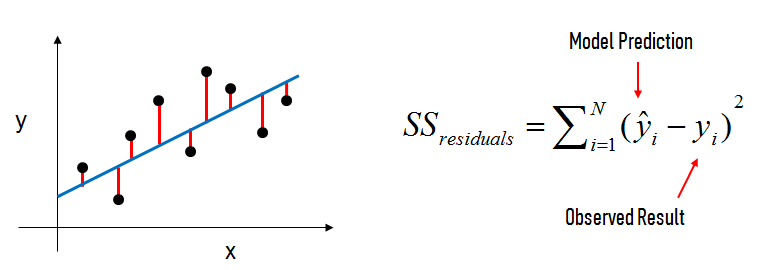
\includegraphics{./assets/estimating_coefficients.png}
\caption{Estimating coefficients}
\end{figure}

In the diagram above:

\begin{itemize}
\tightlist
\item
  The black dots are the \textbf{observed values} of x and y.
\item
  The blue line is our \textbf{least squares line}.
\item
  The red lines are the \textbf{residuals}, which are the vertical
  distances between the observed values and the least squares line.
\end{itemize}

     \#\# Overview of Supervised Learning -\/-\/-

\begin{figure}
\centering
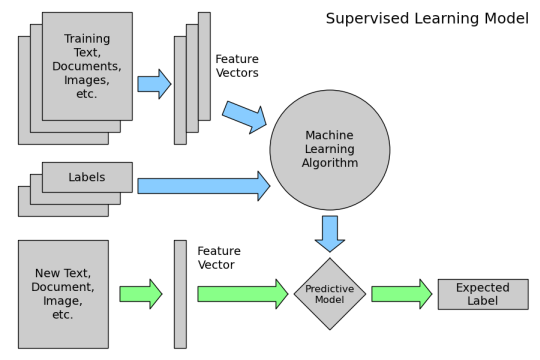
\includegraphics{./assets/supervised_learning.png}
\caption{Supervised learning diagram}
\end{figure}

     \#\#\# Benefits and Drawbacks of scikit-learn

\textbf{Benefits:}

\begin{itemize}
\tightlist
\item
  Consistent interface to machine learning models.
\item
  Provides many tuning parameters but with sensible defaults.
\item
  Exceptional documentation.
\item
  Rich set of functionality for companion tasks.
\item
  Active community for development and support.
\end{itemize}

\textbf{Potential drawbacks:}

\begin{itemize}
\tightlist
\item
  Harder (than R) to get started with machine learning.
\item
  Less emphasis (than R) on model interpretability.

  \begin{itemize}
  \tightlist
  \item
    scikit-learn tends not to run detailed statistical tests, e.g.
    ANOVA.
  \item
    For more detail on model fit, try the \texttt{statsmodels} library.
  \end{itemize}
\end{itemize}

Ben Lorica:
\href{http://radar.oreilly.com/2013/12/six-reasons-why-i-recommend-scikit-learn.html}{Six
Reasons Why I Recommend scikit-learn}

     \#\#\# Requirements for Working With Data in scikit-learn

\begin{enumerate}
\def\labelenumi{\arabic{enumi}.}
\tightlist
\item
  Features and response should be separate objects.
\item
  Features and response should be entirely numeric.
\item
  Features and response should be NumPy arrays (or easily converted to
  NumPy arrays).
\item
  Features and response should have specific shapes (outlined below).
\end{enumerate}

     \#\#\# Building a Linear Regression Model in sklearn

    \paragraph{\texorpdfstring{Create a feature matrix called X that holds a
\texttt{DataFrame} with only the temp variable and a \texttt{Series}
called y that has the "total\_rentals"
column.}{Create a feature matrix called X that holds a DataFrame with only the temp variable and a Series called y that has the "total\_rentals" column.}}\label{create-a-feature-matrix-called-x-that-holds-a-dataframe-with-only-the-temp-variable-and-a-series-called-y-that-has-the-total_rentals-column.}

    \begin{Verbatim}[commandchars=\\\{\}]
{\color{incolor}In [{\color{incolor}13}]:} \PY{c+c1}{\PYZsh{} Create X and y.}
         \PY{n}{feature\PYZus{}cols} \PY{o}{=} \PY{p}{[}\PY{l+s+s1}{\PYZsq{}}\PY{l+s+s1}{temp}\PY{l+s+s1}{\PYZsq{}}\PY{p}{]}
         \PY{n}{X} \PY{o}{=} \PY{n}{bikes}\PY{p}{[}\PY{n}{feature\PYZus{}cols}\PY{p}{]}
         \PY{n}{y} \PY{o}{=} \PY{n}{bikes}\PY{o}{.}\PY{n}{total\PYZus{}rentals}
\end{Verbatim}


    \begin{Verbatim}[commandchars=\\\{\}]
{\color{incolor}In [{\color{incolor}14}]:} \PY{c+c1}{\PYZsh{} Check X\PYZsq{}s type.}
         \PY{n+nb}{print}\PY{p}{(}\PY{p}{(}\PY{n+nb}{type}\PY{p}{(}\PY{n}{X}\PY{p}{)}\PY{p}{)}\PY{p}{)}
         \PY{n+nb}{print}\PY{p}{(}\PY{p}{(}\PY{n+nb}{type}\PY{p}{(}\PY{n}{X}\PY{o}{.}\PY{n}{values}\PY{p}{)}\PY{p}{)}\PY{p}{)}
\end{Verbatim}


    \begin{Verbatim}[commandchars=\\\{\}]
<class 'pandas.core.frame.DataFrame'>
<class 'numpy.ndarray'>

    \end{Verbatim}

    \begin{Verbatim}[commandchars=\\\{\}]
{\color{incolor}In [{\color{incolor}15}]:} \PY{c+c1}{\PYZsh{} Check y\PYZsq{}s type.}
         \PY{n+nb}{print}\PY{p}{(}\PY{p}{(}\PY{n+nb}{type}\PY{p}{(}\PY{n}{y}\PY{p}{)}\PY{p}{)}\PY{p}{)}
         \PY{n+nb}{print}\PY{p}{(}\PY{p}{(}\PY{n+nb}{type}\PY{p}{(}\PY{n}{y}\PY{o}{.}\PY{n}{values}\PY{p}{)}\PY{p}{)}\PY{p}{)}
\end{Verbatim}


    \begin{Verbatim}[commandchars=\\\{\}]
<class 'pandas.core.series.Series'>
<class 'numpy.ndarray'>

    \end{Verbatim}

    \begin{Verbatim}[commandchars=\\\{\}]
{\color{incolor}In [{\color{incolor}16}]:} \PY{c+c1}{\PYZsh{} Check X\PYZsq{}s shape (n = number of observations, m = number of features).}
         \PY{n+nb}{print}\PY{p}{(}\PY{p}{(}\PY{n}{X}\PY{o}{.}\PY{n}{shape}\PY{p}{)}\PY{p}{)}
\end{Verbatim}


    \begin{Verbatim}[commandchars=\\\{\}]
(10886, 1)

    \end{Verbatim}

    \begin{Verbatim}[commandchars=\\\{\}]
{\color{incolor}In [{\color{incolor}17}]:} \PY{c+c1}{\PYZsh{} Check y\PYZsq{}s shape (single dimension with length n).}
         \PY{c+c1}{\PYZsh{} The comma indicates the datatype is a tuple.}
         \PY{n+nb}{print}\PY{p}{(}\PY{p}{(}\PY{n}{y}\PY{o}{.}\PY{n}{shape}\PY{p}{)}\PY{p}{)}
\end{Verbatim}


    \begin{Verbatim}[commandchars=\\\{\}]
(10886,)

    \end{Verbatim}

     \#\#\# scikit-learn's Four-Step Modeling Pattern

    \textbf{Step 1:} Import the class you plan to use.

    \begin{Verbatim}[commandchars=\\\{\}]
{\color{incolor}In [{\color{incolor}18}]:} \PY{k+kn}{from} \PY{n+nn}{sklearn}\PY{n+nn}{.}\PY{n+nn}{linear\PYZus{}model} \PY{k}{import} \PY{n}{LinearRegression}
\end{Verbatim}


    \textbf{Step 2:} "Instantiate" the "estimator."

\begin{itemize}
\tightlist
\item
  "Estimator" is scikit-learn's term for "model."
\item
  "Instantiate" means "make an instance of."
\end{itemize}

    \begin{Verbatim}[commandchars=\\\{\}]
{\color{incolor}In [{\color{incolor}19}]:} \PY{c+c1}{\PYZsh{} Make an instance of a LinearRegression object.}
         \PY{n}{lr} \PY{o}{=} \PY{n}{LinearRegression}\PY{p}{(}\PY{p}{)}
         \PY{n+nb}{type}\PY{p}{(}\PY{n}{lr}\PY{p}{)}
\end{Verbatim}


\begin{Verbatim}[commandchars=\\\{\}]
{\color{outcolor}Out[{\color{outcolor}19}]:} sklearn.linear\_model.base.LinearRegression
\end{Verbatim}
            
    \begin{itemize}
\tightlist
\item
  Created an object that "knows" how to do linear regression, and is
  just waiting for data.
\item
  Name of the object does not matter.
\item
  All parameters not specified are set to their defaults.
\item
  Can specify tuning parameters (aka "hyperparameters") during this
  step.
\end{itemize}

To view the possible parameters, either use the \texttt{help} built-in
function or evaluate the newly instantiated model, as follows:

    \begin{Verbatim}[commandchars=\\\{\}]
{\color{incolor}In [{\color{incolor}20}]:} \PY{c+c1}{\PYZsh{} help(lr)}
         \PY{n}{lr}
\end{Verbatim}


\begin{Verbatim}[commandchars=\\\{\}]
{\color{outcolor}Out[{\color{outcolor}20}]:} LinearRegression(copy\_X=True, fit\_intercept=True, n\_jobs=1, normalize=False)
\end{Verbatim}
            
    \textbf{Step 3:} Fit the model with data (aka "model training").

\begin{itemize}
\tightlist
\item
  Model is "learning" the relationship between X and y in our "training
  data."
\item
  Process through which learning occurs varies by model.
\item
  Occurs in-place.
\end{itemize}

    \begin{Verbatim}[commandchars=\\\{\}]
{\color{incolor}In [{\color{incolor}21}]:} \PY{n}{lr}\PY{o}{.}\PY{n}{fit}\PY{p}{(}\PY{n}{X}\PY{p}{,} \PY{n}{y}\PY{p}{)}
\end{Verbatim}


\begin{Verbatim}[commandchars=\\\{\}]
{\color{outcolor}Out[{\color{outcolor}21}]:} LinearRegression(copy\_X=True, fit\_intercept=True, n\_jobs=1, normalize=False)
\end{Verbatim}
            
    \begin{itemize}
\tightlist
\item
  Once a model has been fit with data, it's called a "fitted model."
\end{itemize}

    \textbf{Step 4:} Predict the response for a new observation.

\begin{itemize}
\tightlist
\item
  New observations are called "out-of-sample" data.
\item
  Uses the information it learned during the model training process.
\end{itemize}

    \begin{Verbatim}[commandchars=\\\{\}]
{\color{incolor}In [{\color{incolor}22}]:} \PY{c+c1}{\PYZsh{} Per future warning, one\PYZhy{}dimensional arrays must be reshaped using the following.}
         \PY{n}{lr}\PY{o}{.}\PY{n}{predict}\PY{p}{(}\PY{n}{np}\PY{o}{.}\PY{n}{array}\PY{p}{(}\PY{p}{[}\PY{l+m+mi}{0}\PY{p}{]}\PY{p}{)}\PY{o}{.}\PY{n}{reshape}\PY{p}{(}\PY{l+m+mi}{1}\PY{p}{,}\PY{o}{\PYZhy{}}\PY{l+m+mi}{1}\PY{p}{)}\PY{p}{)}
\end{Verbatim}


\begin{Verbatim}[commandchars=\\\{\}]
{\color{outcolor}Out[{\color{outcolor}22}]:} array([6.04621296])
\end{Verbatim}
            
    Let's ask the model to make two predictions, one when the \texttt{temp}
is 0 and another when the \texttt{temp} is 10. To do this, our feature
matrix is always a 2-D array where each row is a list of features. Since
we only have a single feature, the temperature, each row will contain
only a single value.

    \begin{Verbatim}[commandchars=\\\{\}]
{\color{incolor}In [{\color{incolor}23}]:} \PY{n}{X\PYZus{}new} \PY{o}{=} \PY{p}{[}\PY{p}{[}\PY{l+m+mi}{0}\PY{p}{]}\PY{p}{,} \PY{p}{[}\PY{l+m+mi}{10}\PY{p}{]}\PY{p}{]}
         \PY{n}{lr}\PY{o}{.}\PY{n}{predict}\PY{p}{(}\PY{n}{X\PYZus{}new}\PY{p}{)}
\end{Verbatim}


\begin{Verbatim}[commandchars=\\\{\}]
{\color{outcolor}Out[{\color{outcolor}23}]:} array([ 6.04621296, 97.75161777])
\end{Verbatim}
            
    \begin{itemize}
\tightlist
\item
  Returns a NumPy array, and we keep track of what the numbers "mean."
\item
  Can predict for multiple observations at once.
\end{itemize}

    What we just predicted using our model is, "If the temperature is 0
degrees, the total number of bike rentals will be
\textasciitilde{}6.046, and if the temperature is 10 degrees the total
number of bike rentals will \textasciitilde{}97.751."

     \#\# Build a Linear Regression Model -\/-\/-

    Let's specifically make a linear regression model and look at the
intercept and coefficients.

    \paragraph{\texorpdfstring{Instantiate and fit a
\texttt{LinearRegression} model on X and y from the
\texttt{linear\_model} section of
scikit-learn.}{Instantiate and fit a LinearRegression model on X and y from the linear\_model section of scikit-learn.}}\label{instantiate-and-fit-a-linearregression-model-on-x-and-y-from-the-linear_model-section-of-scikit-learn.}

    \begin{Verbatim}[commandchars=\\\{\}]
{\color{incolor}In [{\color{incolor}24}]:} \PY{c+c1}{\PYZsh{} Import, instantiate, fit.}
         \PY{k+kn}{from} \PY{n+nn}{sklearn}\PY{n+nn}{.}\PY{n+nn}{linear\PYZus{}model} \PY{k}{import} \PY{n}{LinearRegression}
         \PY{n}{linreg} \PY{o}{=} \PY{n}{LinearRegression}\PY{p}{(}\PY{p}{)}
         \PY{n}{linreg}\PY{o}{.}\PY{n}{fit}\PY{p}{(}\PY{n}{X}\PY{p}{,} \PY{n}{y}\PY{p}{)}
\end{Verbatim}


\begin{Verbatim}[commandchars=\\\{\}]
{\color{outcolor}Out[{\color{outcolor}24}]:} LinearRegression(copy\_X=True, fit\_intercept=True, n\_jobs=1, normalize=False)
\end{Verbatim}
            
    \begin{Verbatim}[commandchars=\\\{\}]
{\color{incolor}In [{\color{incolor}25}]:} \PY{c+c1}{\PYZsh{} Print the coefficients.}
         \PY{n+nb}{print}\PY{p}{(}\PY{n}{linreg}\PY{o}{.}\PY{n}{intercept\PYZus{}}\PY{p}{)}
         \PY{n+nb}{print}\PY{p}{(}\PY{n}{linreg}\PY{o}{.}\PY{n}{coef\PYZus{}}\PY{p}{)}
\end{Verbatim}


    \begin{Verbatim}[commandchars=\\\{\}]
6.046212959616781
[9.17054048]

    \end{Verbatim}

    Interpreting the intercept (\(\beta_0\)):

\begin{itemize}
\tightlist
\item
  It is the value of \(y\) when all independent variables are 0.
\item
  Here, it is the estimated number of rentals when the temperature is 0
  degrees Celsius.
\item
  \textbf{Note:} It does not always make sense to interpret the
  intercept. (Why?)
\end{itemize}

Interpreting the "temp" coefficient (\(\beta_1\)):

\begin{itemize}
\tightlist
\item
  \textbf{Interpretation:} An increase of 1 degree Celcius is
  \emph{associated with} increasing the number of total rentals by
  \(\beta_1\).
\item
  Here, a temperature increase of 1 degree Celsius is \emph{associated
  with} a rental increase of 9.17 bikes.
\item
  This is not a statement of causation.
\item
  \(\beta_1\) would be \textbf{negative} if an increase in temperature
  was associated with a \textbf{decrease} in total rentals.
\item
  \(\beta_1\) would be \textbf{zero} if temperature is not associated
  with total rentals.
\end{itemize}

     \#\# Using the Model for Prediction -\/-\/-

While plenty of insight can be found in reading coefficients, the most
common uses of data science focus on prediction. In scikit-learn we can
make predictions from a fitted model using \texttt{.predict()}, but we
will also go through the calculation by hand to understand it.

    \paragraph{How many bike rentals would we predict if the temperature was
25 degrees
Celsius?}\label{how-many-bike-rentals-would-we-predict-if-the-temperature-was-25-degrees-celsius}

    \paragraph{Explore the intercept and coefficients of the linear
model.}\label{explore-the-intercept-and-coefficients-of-the-linear-model.}

You can search for "sklearn linear regression" and explore the
attributes section of the documentation to learn how to do this.

    \begin{Verbatim}[commandchars=\\\{\}]
{\color{incolor}In [{\color{incolor}26}]:} \PY{c+c1}{\PYZsh{} Manually calculate the prediction.}
         \PY{k}{def} \PY{n+nf}{predict\PYZus{}rentals}\PY{p}{(}\PY{n}{temp}\PY{p}{)}\PY{p}{:}
             \PY{k}{return} \PY{n}{linreg}\PY{o}{.}\PY{n}{intercept\PYZus{}} \PY{o}{+} \PY{p}{(}\PY{n}{linreg}\PY{o}{.}\PY{n}{coef\PYZus{}}\PY{p}{[}\PY{l+m+mi}{0}\PY{p}{]}\PY{o}{*}\PY{n}{temp}\PY{p}{)}
         
         \PY{n}{predict\PYZus{}rentals}\PY{p}{(}\PY{l+m+mi}{90}\PY{p}{)}
\end{Verbatim}


\begin{Verbatim}[commandchars=\\\{\}]
{\color{outcolor}Out[{\color{outcolor}26}]:} 831.3948562879783
\end{Verbatim}
            
    \begin{Verbatim}[commandchars=\\\{\}]
{\color{incolor}In [{\color{incolor}27}]:} \PY{c+c1}{\PYZsh{} Use the predict method.}
         \PY{n}{lr}\PY{o}{.}\PY{n}{predict}\PY{p}{(}\PY{l+m+mi}{90}\PY{p}{)}
\end{Verbatim}


\begin{Verbatim}[commandchars=\\\{\}]
{\color{outcolor}Out[{\color{outcolor}27}]:} array([831.39485629])
\end{Verbatim}
            
     \#\#\# Does the Scale of the Features Matter?

Let's say that temperature was measured in Fahrenheit, rather than
Celsius. How would that affect the model?

    \begin{Verbatim}[commandchars=\\\{\}]
{\color{incolor}In [{\color{incolor}28}]:} \PY{c+c1}{\PYZsh{} Create a new column for Fahrenheit temperature.}
         \PY{n}{bikes}\PY{p}{[}\PY{l+s+s1}{\PYZsq{}}\PY{l+s+s1}{temp\PYZus{}F}\PY{l+s+s1}{\PYZsq{}}\PY{p}{]} \PY{o}{=} \PY{n}{bikes}\PY{o}{.}\PY{n}{temp} \PY{o}{*} \PY{l+m+mf}{1.8} \PY{o}{+} \PY{l+m+mi}{32}
         \PY{n}{bikes}\PY{o}{.}\PY{n}{head}\PY{p}{(}\PY{p}{)}
\end{Verbatim}


\begin{Verbatim}[commandchars=\\\{\}]
{\color{outcolor}Out[{\color{outcolor}28}]:}                      season  holiday  workingday  weather  temp   atemp  \textbackslash{}
         datetime                                                                  
         2011-01-01 00:00:00       1        0           0        1  9.84  14.395   
         2011-01-01 01:00:00       1        0           0        1  9.02  13.635   
         2011-01-01 02:00:00       1        0           0        1  9.02  13.635   
         2011-01-01 03:00:00       1        0           0        1  9.84  14.395   
         2011-01-01 04:00:00       1        0           0        1  9.84  14.395   
         
                              humidity  windspeed  casual  registered  total\_rentals  \textbackslash{}
         datetime                                                                      
         2011-01-01 00:00:00        81        0.0       3          13             16   
         2011-01-01 01:00:00        80        0.0       8          32             40   
         2011-01-01 02:00:00        80        0.0       5          27             32   
         2011-01-01 03:00:00        75        0.0       3          10             13   
         2011-01-01 04:00:00        75        0.0       0           1              1   
         
                              temp\_F  
         datetime                     
         2011-01-01 00:00:00  49.712  
         2011-01-01 01:00:00  48.236  
         2011-01-01 02:00:00  48.236  
         2011-01-01 03:00:00  49.712  
         2011-01-01 04:00:00  49.712  
\end{Verbatim}
            
    \begin{Verbatim}[commandchars=\\\{\}]
{\color{incolor}In [{\color{incolor}29}]:} \PY{c+c1}{\PYZsh{} Seaborn scatterplot with regression line}
         \PY{n}{sns}\PY{o}{.}\PY{n}{lmplot}\PY{p}{(}\PY{n}{x}\PY{o}{=}\PY{l+s+s1}{\PYZsq{}}\PY{l+s+s1}{temp\PYZus{}F}\PY{l+s+s1}{\PYZsq{}}\PY{p}{,} \PY{n}{y}\PY{o}{=}\PY{l+s+s1}{\PYZsq{}}\PY{l+s+s1}{total\PYZus{}rentals}\PY{l+s+s1}{\PYZsq{}}\PY{p}{,} \PY{n}{data}\PY{o}{=}\PY{n}{bikes}\PY{p}{,} \PY{n}{aspect}\PY{o}{=}\PY{l+m+mf}{1.5}\PY{p}{,} \PY{n}{scatter\PYZus{}kws}\PY{o}{=}\PY{p}{\PYZob{}}\PY{l+s+s1}{\PYZsq{}}\PY{l+s+s1}{alpha}\PY{l+s+s1}{\PYZsq{}}\PY{p}{:}\PY{l+m+mf}{0.2}\PY{p}{\PYZcb{}}\PY{p}{)}\PY{p}{;}
\end{Verbatim}


    \begin{Verbatim}[commandchars=\\\{\}]
/anaconda2/envs/py36/lib/python3.6/site-packages/scipy/stats/stats.py:1713: FutureWarning: Using a non-tuple sequence for multidimensional indexing is deprecated; use `arr[tuple(seq)]` instead of `arr[seq]`. In the future this will be interpreted as an array index, `arr[np.array(seq)]`, which will result either in an error or a different result.
  return np.add.reduce(sorted[indexer] * weights, axis=axis) / sumval

    \end{Verbatim}

    \begin{center}
    \adjustimage{max size={0.9\linewidth}{0.9\paperheight}}{output_67_1.png}
    \end{center}
    { \hspace*{\fill} \\}
    
    \paragraph{\texorpdfstring{Rebuild the \texttt{LinearRegression} from
above using the \texttt{temp\_F} features
instead.}{Rebuild the LinearRegression from above using the temp\_F features instead.}}\label{rebuild-the-linearregression-from-above-using-the-temp_f-features-instead.}

    \begin{Verbatim}[commandchars=\\\{\}]
{\color{incolor}In [{\color{incolor}30}]:} \PY{c+c1}{\PYZsh{} Create X and y.}
         \PY{n}{feature\PYZus{}cols} \PY{o}{=} \PY{p}{[}\PY{l+s+s1}{\PYZsq{}}\PY{l+s+s1}{temp\PYZus{}F}\PY{l+s+s1}{\PYZsq{}}\PY{p}{]}
         \PY{n}{X} \PY{o}{=} \PY{n}{bikes}\PY{p}{[}\PY{n}{feature\PYZus{}cols}\PY{p}{]}
         \PY{n}{y} \PY{o}{=} \PY{n}{bikes}\PY{o}{.}\PY{n}{total\PYZus{}rentals}
         
         \PY{c+c1}{\PYZsh{} Instantiate and fit.}
         \PY{n}{linreg} \PY{o}{=} \PY{n}{LinearRegression}\PY{p}{(}\PY{p}{)}
         \PY{n}{linreg}\PY{o}{.}\PY{n}{fit}\PY{p}{(}\PY{n}{X}\PY{p}{,} \PY{n}{y}\PY{p}{)}
         
         \PY{c+c1}{\PYZsh{} Print the coefficients.}
         \PY{n+nb}{print}\PY{p}{(}\PY{n}{linreg}\PY{o}{.}\PY{n}{intercept\PYZus{}}\PY{p}{)}
         \PY{n+nb}{print}\PY{p}{(}\PY{n}{linreg}\PY{o}{.}\PY{n}{coef\PYZus{}}\PY{p}{)}
\end{Verbatim}


    \begin{Verbatim}[commandchars=\\\{\}]
-156.98561782129445
[5.09474471]

    \end{Verbatim}

    \paragraph{Convert 25 degrees Celsius to
Fahrenheit.}\label{convert-25-degrees-celsius-to-fahrenheit.}

    \begin{Verbatim}[commandchars=\\\{\}]
{\color{incolor}In [{\color{incolor}31}]:} \PY{l+m+mi}{25} \PY{o}{*} \PY{l+m+mf}{1.8} \PY{o}{+} \PY{l+m+mi}{32}
\end{Verbatim}


\begin{Verbatim}[commandchars=\\\{\}]
{\color{outcolor}Out[{\color{outcolor}31}]:} 77.0
\end{Verbatim}
            
    \paragraph{Predict rentals for 77 degrees
Fahrenheit.}\label{predict-rentals-for-77-degrees-fahrenheit.}

    \begin{Verbatim}[commandchars=\\\{\}]
{\color{incolor}In [{\color{incolor}32}]:} \PY{n}{linreg}\PY{o}{.}\PY{n}{predict}\PY{p}{(}\PY{l+m+mi}{77}\PY{p}{)}
\end{Verbatim}


\begin{Verbatim}[commandchars=\\\{\}]
{\color{outcolor}Out[{\color{outcolor}32}]:} array([235.309725])
\end{Verbatim}
            
    \textbf{Conclusion:} The scale of the features is irrelevant for linear
regression models. When changing the scale, we simply change our
interpretation of the coefficients.

    \begin{Verbatim}[commandchars=\\\{\}]
{\color{incolor}In [{\color{incolor}33}]:} \PY{c+c1}{\PYZsh{} Remove the temp\PYZus{}F column.}
         \PY{n}{bikes}\PY{o}{.}\PY{n}{drop}\PY{p}{(}\PY{l+s+s1}{\PYZsq{}}\PY{l+s+s1}{temp\PYZus{}F}\PY{l+s+s1}{\PYZsq{}}\PY{p}{,} \PY{n}{axis}\PY{o}{=}\PY{l+m+mi}{1}\PY{p}{,} \PY{n}{inplace}\PY{o}{=}\PY{k+kc}{True}\PY{p}{)}
\end{Verbatim}


     \#\# Work With Multiple Features -\/-\/-

We've demonstrated simple linear regression with one feature to gain an
intuition, but the benefit of modeling is the ability to reason about
hundreds of features at once. There is no limit to the number of
features you can use. However, often a small set of features accounts
for most of the variance (assuming there is a linear relationship at
all). We will start by using four features.

     \#\#\# Visualizing the Data (Part 2)

    \paragraph{Explore more features.}\label{explore-more-features.}

    \begin{Verbatim}[commandchars=\\\{\}]
{\color{incolor}In [{\color{incolor}34}]:} \PY{c+c1}{\PYZsh{} Create feature column variables}
         \PY{n}{feature\PYZus{}cols} \PY{o}{=} \PY{p}{[}\PY{l+s+s1}{\PYZsq{}}\PY{l+s+s1}{temp}\PY{l+s+s1}{\PYZsq{}}\PY{p}{,} \PY{l+s+s1}{\PYZsq{}}\PY{l+s+s1}{season}\PY{l+s+s1}{\PYZsq{}}\PY{p}{,} \PY{l+s+s1}{\PYZsq{}}\PY{l+s+s1}{weather}\PY{l+s+s1}{\PYZsq{}}\PY{p}{,} \PY{l+s+s1}{\PYZsq{}}\PY{l+s+s1}{humidity}\PY{l+s+s1}{\PYZsq{}}\PY{p}{]}
\end{Verbatim}


    \paragraph{Create a subset of scatterplot matrix using
Seaborn.}\label{create-a-subset-of-scatterplot-matrix-using-seaborn.}

We can use pairplot with the y\_vars argument to only show relationships
with the \texttt{total\_rentals} variable

    \begin{Verbatim}[commandchars=\\\{\}]
{\color{incolor}In [{\color{incolor}35}]:} \PY{c+c1}{\PYZsh{} multiple scatterplots in Seaborn}
         \PY{n}{sns}\PY{o}{.}\PY{n}{pairplot}\PY{p}{(}\PY{n}{bikes}\PY{p}{,} \PY{n}{x\PYZus{}vars}\PY{o}{=}\PY{n}{feature\PYZus{}cols}\PY{p}{,} 
                      \PY{n}{y\PYZus{}vars}\PY{o}{=}\PY{l+s+s1}{\PYZsq{}}\PY{l+s+s1}{total\PYZus{}rentals}\PY{l+s+s1}{\PYZsq{}}\PY{p}{,} \PY{n}{kind}\PY{o}{=}\PY{l+s+s1}{\PYZsq{}}\PY{l+s+s1}{reg}\PY{l+s+s1}{\PYZsq{}}\PY{p}{)}\PY{p}{;}
\end{Verbatim}


    \begin{Verbatim}[commandchars=\\\{\}]
/anaconda2/envs/py36/lib/python3.6/site-packages/scipy/stats/stats.py:1713: FutureWarning: Using a non-tuple sequence for multidimensional indexing is deprecated; use `arr[tuple(seq)]` instead of `arr[seq]`. In the future this will be interpreted as an array index, `arr[np.array(seq)]`, which will result either in an error or a different result.
  return np.add.reduce(sorted[indexer] * weights, axis=axis) / sumval

    \end{Verbatim}

    \begin{center}
    \adjustimage{max size={0.9\linewidth}{0.9\paperheight}}{output_81_1.png}
    \end{center}
    { \hspace*{\fill} \\}
    
    \paragraph{Recreate the same functionality using
Pandas.}\label{recreate-the-same-functionality-using-pandas.}

    \begin{Verbatim}[commandchars=\\\{\}]
{\color{incolor}In [{\color{incolor}36}]:} \PY{c+c1}{\PYZsh{} Multiple scatterplots in Pandas}
         \PY{n}{fig}\PY{p}{,} \PY{n}{axs} \PY{o}{=} \PY{n}{plt}\PY{o}{.}\PY{n}{subplots}\PY{p}{(}\PY{l+m+mi}{1}\PY{p}{,} \PY{n+nb}{len}\PY{p}{(}\PY{n}{feature\PYZus{}cols}\PY{p}{)}\PY{p}{,} \PY{n}{sharey}\PY{o}{=}\PY{k+kc}{True}\PY{p}{)}
         \PY{k}{for} \PY{n}{index}\PY{p}{,} \PY{n}{feature} \PY{o+ow}{in} \PY{n+nb}{enumerate}\PY{p}{(}\PY{n}{feature\PYZus{}cols}\PY{p}{)}\PY{p}{:}
             \PY{n}{bikes}\PY{o}{.}\PY{n}{plot}\PY{p}{(}\PY{n}{kind}\PY{o}{=}\PY{l+s+s1}{\PYZsq{}}\PY{l+s+s1}{scatter}\PY{l+s+s1}{\PYZsq{}}\PY{p}{,} \PY{n}{x}\PY{o}{=}\PY{n}{feature}\PY{p}{,} \PY{n}{y}\PY{o}{=}\PY{l+s+s1}{\PYZsq{}}\PY{l+s+s1}{total\PYZus{}rentals}\PY{l+s+s1}{\PYZsq{}}\PY{p}{,} 
                        \PY{n}{ax}\PY{o}{=}\PY{n}{axs}\PY{p}{[}\PY{n}{index}\PY{p}{]}\PY{p}{,} \PY{n}{figsize}\PY{o}{=}\PY{p}{(}\PY{l+m+mi}{16}\PY{p}{,} \PY{l+m+mi}{3}\PY{p}{)}\PY{p}{)}
\end{Verbatim}


    \begin{center}
    \adjustimage{max size={0.9\linewidth}{0.9\paperheight}}{output_83_0.png}
    \end{center}
    { \hspace*{\fill} \\}
    
    \begin{Verbatim}[commandchars=\\\{\}]
{\color{incolor}In [{\color{incolor}37}]:} \PY{c+c1}{\PYZsh{} alternative way in Pandas (might take a while)}
         \PY{c+c1}{\PYZsh{} scatter\PYZus{}matrix does a pairplot of *every* column}
         
         \PY{n}{grr} \PY{o}{=} \PY{n}{pd}\PY{o}{.}\PY{n}{tools}\PY{o}{.}\PY{n}{plotting}\PY{o}{.}\PY{n}{scatter\PYZus{}matrix}\PY{p}{(}
             \PY{n}{bikes}\PY{p}{[}\PY{p}{[}\PY{l+s+s1}{\PYZsq{}}\PY{l+s+s1}{total\PYZus{}rentals}\PY{l+s+s1}{\PYZsq{}}\PY{p}{]} \PY{o}{+} \PY{n}{feature\PYZus{}cols}\PY{p}{]}\PY{p}{,} 
             \PY{n}{figsize}\PY{o}{=}\PY{p}{(}\PY{l+m+mi}{15}\PY{p}{,} \PY{l+m+mi}{15}\PY{p}{)}\PY{p}{,} \PY{n}{alpha}\PY{o}{=}\PY{l+m+mf}{0.7}\PY{p}{)}
\end{Verbatim}


    \begin{Verbatim}[commandchars=\\\{\}]
/anaconda2/envs/py36/lib/python3.6/site-packages/ipykernel/\_\_main\_\_.py:6: FutureWarning: 'pandas.tools.plotting.scatter\_matrix' is deprecated, import 'pandas.plotting.scatter\_matrix' instead.

    \end{Verbatim}

    \begin{center}
    \adjustimage{max size={0.9\linewidth}{0.9\paperheight}}{output_84_1.png}
    \end{center}
    { \hspace*{\fill} \\}
    
    \paragraph{Are you seeing anything you didn't
expect?}\label{are-you-seeing-anything-you-didnt-expect}

    \paragraph{Explore the season variable using a
cross-tab.}\label{explore-the-season-variable-using-a-cross-tab.}

    \begin{Verbatim}[commandchars=\\\{\}]
{\color{incolor}In [{\color{incolor}38}]:} \PY{c+c1}{\PYZsh{} Cross\PYZhy{}tabulation of season and month}
         \PY{n}{pd}\PY{o}{.}\PY{n}{crosstab}\PY{p}{(}\PY{n}{bikes}\PY{o}{.}\PY{n}{season}\PY{p}{,} \PY{n}{bikes}\PY{o}{.}\PY{n}{index}\PY{o}{.}\PY{n}{month}\PY{p}{)}
\end{Verbatim}


\begin{Verbatim}[commandchars=\\\{\}]
{\color{outcolor}Out[{\color{outcolor}38}]:} col\_0    1    2    3    4    5    6    7    8    9    10   11   12
         season                                                            
         1       884  901  901    0    0    0    0    0    0    0    0    0
         2         0    0    0  909  912  912    0    0    0    0    0    0
         3         0    0    0    0    0    0  912  912  909    0    0    0
         4         0    0    0    0    0    0    0    0    0  911  911  912
\end{Verbatim}
            
    \paragraph{Explore the season variable using a box
plot.}\label{explore-the-season-variable-using-a-box-plot.}

    \begin{Verbatim}[commandchars=\\\{\}]
{\color{incolor}In [{\color{incolor}39}]:} \PY{c+c1}{\PYZsh{} Box plot of rentals, grouped by season}
         \PY{n}{bikes}\PY{o}{.}\PY{n}{boxplot}\PY{p}{(}\PY{n}{column}\PY{o}{=}\PY{l+s+s1}{\PYZsq{}}\PY{l+s+s1}{total\PYZus{}rentals}\PY{l+s+s1}{\PYZsq{}}\PY{p}{,} \PY{n}{by}\PY{o}{=}\PY{l+s+s1}{\PYZsq{}}\PY{l+s+s1}{season}\PY{l+s+s1}{\PYZsq{}}\PY{p}{)}\PY{p}{;}
\end{Verbatim}


    \begin{center}
    \adjustimage{max size={0.9\linewidth}{0.9\paperheight}}{output_89_0.png}
    \end{center}
    { \hspace*{\fill} \\}
    
    Notably:

\begin{itemize}
\tightlist
\item
  A line can't capture a nonlinear relationship.
\end{itemize}

    \paragraph{Look at rentals over time.}\label{look-at-rentals-over-time.}

    \begin{Verbatim}[commandchars=\\\{\}]
{\color{incolor}In [{\color{incolor}40}]:} \PY{c+c1}{\PYZsh{} Line plot of rentals}
         \PY{n}{bikes}\PY{o}{.}\PY{n}{total\PYZus{}rentals}\PY{o}{.}\PY{n}{plot}\PY{p}{(}\PY{p}{)}\PY{p}{;}
\end{Verbatim}


    \begin{center}
    \adjustimage{max size={0.9\linewidth}{0.9\paperheight}}{output_92_0.png}
    \end{center}
    { \hspace*{\fill} \\}
    
    \paragraph{What does this tell us?}\label{what-does-this-tell-us}

There are more rentals in the winter than the spring, but only because
the system is experiencing overall growth and the winter months happen
to come after the spring months.

    \paragraph{\texorpdfstring{Look at the correlation matrix for the bikes
\texttt{DataFrame}.}{Look at the correlation matrix for the bikes DataFrame.}}\label{look-at-the-correlation-matrix-for-the-bikes-dataframe.}

    \begin{Verbatim}[commandchars=\\\{\}]
{\color{incolor}In [{\color{incolor}41}]:} \PY{c+c1}{\PYZsh{} Correlation matrix (ranges from 1 to \PYZhy{}1)}
         \PY{n}{bikes}\PY{o}{.}\PY{n}{corr}\PY{p}{(}\PY{p}{)}\PY{o}{.}\PY{n}{style}\PY{o}{.}\PY{n}{background\PYZus{}gradient}\PY{p}{(}\PY{p}{)}
\end{Verbatim}


\begin{Verbatim}[commandchars=\\\{\}]
{\color{outcolor}Out[{\color{outcolor}41}]:} <pandas.io.formats.style.Styler at 0x1a19dd1320>
\end{Verbatim}
            
    \paragraph{Use a heat map to make it easier to read the correlation
matrix.}\label{use-a-heat-map-to-make-it-easier-to-read-the-correlation-matrix.}

    \begin{Verbatim}[commandchars=\\\{\}]
{\color{incolor}In [{\color{incolor}42}]:} \PY{c+c1}{\PYZsh{} Visualize correlation matrix in Seaborn using a heat map.}
         \PY{n}{sns}\PY{o}{.}\PY{n}{heatmap}\PY{p}{(}\PY{n}{bikes}\PY{o}{.}\PY{n}{corr}\PY{p}{(}\PY{p}{)}\PY{p}{)}
\end{Verbatim}


\begin{Verbatim}[commandchars=\\\{\}]
{\color{outcolor}Out[{\color{outcolor}42}]:} <matplotlib.axes.\_subplots.AxesSubplot at 0x1a188eb4a8>
\end{Verbatim}
            
    \begin{center}
    \adjustimage{max size={0.9\linewidth}{0.9\paperheight}}{output_97_1.png}
    \end{center}
    { \hspace*{\fill} \\}
    
    \paragraph{What relationships do you
notice?}\label{what-relationships-do-you-notice}

    \begin{Verbatim}[commandchars=\\\{\}]
{\color{incolor}In [{\color{incolor}43}]:} \PY{c+c1}{\PYZsh{} A:}
\end{Verbatim}


     \#\#\# Adding More Features to the Model

    In the previous example, one variable explained the variance of another;
however, more often than not, we will need multiple variables.

\begin{itemize}
\item
  For example, a house's price may be best measured by square feet, but
  a lot of other variables play a vital role: bedrooms, bathrooms,
  location, appliances, etc.
\item
  For a linear regression, we want these variables to be largely
  independent of one another, but all of them should help explain the y
  variable.
\end{itemize}

We'll work with bikeshare data to showcase what this means and to
explain a concept called multicollinearity.

    \paragraph{\texorpdfstring{Create another \texttt{LinearRegression}
instance that is fit using temp, season, weather, and
humidity.}{Create another LinearRegression instance that is fit using temp, season, weather, and humidity.}}\label{create-another-linearregression-instance-that-is-fit-using-temp-season-weather-and-humidity.}

    \begin{Verbatim}[commandchars=\\\{\}]
{\color{incolor}In [{\color{incolor}44}]:} \PY{c+c1}{\PYZsh{} Create a list of features.}
         \PY{n}{feature\PYZus{}cols} \PY{o}{=} \PY{p}{[}\PY{l+s+s1}{\PYZsq{}}\PY{l+s+s1}{temp}\PY{l+s+s1}{\PYZsq{}}\PY{p}{,} \PY{l+s+s1}{\PYZsq{}}\PY{l+s+s1}{season}\PY{l+s+s1}{\PYZsq{}}\PY{p}{,} \PY{l+s+s1}{\PYZsq{}}\PY{l+s+s1}{weather}\PY{l+s+s1}{\PYZsq{}}\PY{p}{,} \PY{l+s+s1}{\PYZsq{}}\PY{l+s+s1}{humidity}\PY{l+s+s1}{\PYZsq{}}\PY{p}{]}
\end{Verbatim}


    \begin{Verbatim}[commandchars=\\\{\}]
{\color{incolor}In [{\color{incolor}45}]:} \PY{c+c1}{\PYZsh{} Create X and y.}
         \PY{n}{X} \PY{o}{=} \PY{n}{bikes}\PY{p}{[}\PY{n}{feature\PYZus{}cols}\PY{p}{]}
         \PY{n}{y} \PY{o}{=} \PY{n}{bikes}\PY{o}{.}\PY{n}{total\PYZus{}rentals}
         
         \PY{c+c1}{\PYZsh{} Instantiate and fit.}
         \PY{n}{linreg} \PY{o}{=} \PY{n}{LinearRegression}\PY{p}{(}\PY{p}{)}
         \PY{n}{linreg}\PY{o}{.}\PY{n}{fit}\PY{p}{(}\PY{n}{X}\PY{p}{,} \PY{n}{y}\PY{p}{)}
         
         \PY{c+c1}{\PYZsh{} Print the coefficients.}
         \PY{n+nb}{print}\PY{p}{(}\PY{n}{linreg}\PY{o}{.}\PY{n}{intercept\PYZus{}}\PY{p}{)}
         \PY{n+nb}{print}\PY{p}{(}\PY{n}{linreg}\PY{o}{.}\PY{n}{coef\PYZus{}}\PY{p}{)}
\end{Verbatim}


    \begin{Verbatim}[commandchars=\\\{\}]
159.52068786129817
[ 7.86482499 22.53875753  6.67030204 -3.11887338]

    \end{Verbatim}

    \paragraph{Display the linear regression coefficient along with the
feature
names.}\label{display-the-linear-regression-coefficient-along-with-the-feature-names.}

    \begin{Verbatim}[commandchars=\\\{\}]
{\color{incolor}In [{\color{incolor}46}]:} \PY{c+c1}{\PYZsh{} Pair the feature names with the coefficients.}
         \PY{n+nb}{list}\PY{p}{(}\PY{n+nb}{zip}\PY{p}{(}\PY{n}{feature\PYZus{}cols}\PY{p}{,} \PY{n}{linreg}\PY{o}{.}\PY{n}{coef\PYZus{}}\PY{p}{)}\PY{p}{)}
\end{Verbatim}


\begin{Verbatim}[commandchars=\\\{\}]
{\color{outcolor}Out[{\color{outcolor}46}]:} [('temp', 7.864824992477439),
          ('season', 22.53875753246676),
          ('weather', 6.670302035923719),
          ('humidity', -3.118873382396501)]
\end{Verbatim}
            
    Interpreting the coefficients:

\begin{itemize}
\tightlist
\item
  Holding all other features fixed, a 1-unit increase in temperature is
  associated with a rental increase of 7.86 bikes.
\item
  Holding all other features fixed, a 1-unit increase in season is
  associated with a rental increase of 22.5 bikes.
\item
  Holding all other features fixed, a 1-unit increase in weather is
  associated with a rental increase of 6.67 bikes.
\item
  Holding all other features fixed, a 1-unit increase in humidity is
  associated with a rental decrease of 3.12 bikes.
\end{itemize}

Does anything look incorrect and does not reflect reality?

     \#\# What Is Multicollinearity? -\/-\/-

Multicollinearity happens when two or more features are highly
correlated with each other. The problem is that due to the high
correlation, it's hard to disambiguate which feature has what kind of
effect on the outcome. In other words, the features mask each other.

There is a second related issue called variance inflation where
including correlated features increases the variability of our model and
p-values by widening the standard errors. This can be measured with the
variance inflation factor, which we will not cover here.

    \paragraph{With the bikeshare data, let's compare three data points:
actual temperature, "feel" temperature, and guest
ridership.}\label{with-the-bikeshare-data-lets-compare-three-data-points-actual-temperature-feel-temperature-and-guest-ridership.}

    \begin{Verbatim}[commandchars=\\\{\}]
{\color{incolor}In [{\color{incolor}47}]:} \PY{n}{cmap} \PY{o}{=} \PY{n}{sns}\PY{o}{.}\PY{n}{diverging\PYZus{}palette}\PY{p}{(}\PY{l+m+mi}{220}\PY{p}{,} \PY{l+m+mi}{10}\PY{p}{,} \PY{n}{as\PYZus{}cmap}\PY{o}{=}\PY{k+kc}{True}\PY{p}{)}
         \PY{n}{correlations} \PY{o}{=} \PY{n}{bikes}\PY{p}{[}\PY{p}{[}\PY{l+s+s1}{\PYZsq{}}\PY{l+s+s1}{temp}\PY{l+s+s1}{\PYZsq{}}\PY{p}{,} \PY{l+s+s1}{\PYZsq{}}\PY{l+s+s1}{atemp}\PY{l+s+s1}{\PYZsq{}}\PY{p}{,} \PY{l+s+s1}{\PYZsq{}}\PY{l+s+s1}{casual}\PY{l+s+s1}{\PYZsq{}}\PY{p}{]}\PY{p}{]}\PY{o}{.}\PY{n}{corr}\PY{p}{(}\PY{p}{)}
         \PY{n+nb}{print}\PY{p}{(}\PY{n}{correlations}\PY{p}{)}
         \PY{n+nb}{print}\PY{p}{(}\PY{n}{sns}\PY{o}{.}\PY{n}{heatmap}\PY{p}{(}\PY{n}{correlations}\PY{p}{,} \PY{n}{cmap}\PY{o}{=}\PY{n}{cmap}\PY{p}{)}\PY{p}{)}
\end{Verbatim}


    \begin{Verbatim}[commandchars=\\\{\}]
            temp     atemp    casual
temp    1.000000  0.984948  0.467097
atemp   0.984948  1.000000  0.462067
casual  0.467097  0.462067  1.000000
AxesSubplot(0.08,0.125;0.696x0.755)

    \end{Verbatim}

    \begin{center}
    \adjustimage{max size={0.9\linewidth}{0.9\paperheight}}{output_110_1.png}
    \end{center}
    { \hspace*{\fill} \\}
    
    \paragraph{\texorpdfstring{Create a linear model that predicts
\texttt{total\_rentals} using \texttt{temp} and
\texttt{atemp}.}{Create a linear model that predicts total\_rentals using temp and atemp.}}\label{create-a-linear-model-that-predicts-total_rentals-using-temp-and-atemp.}

    \begin{Verbatim}[commandchars=\\\{\}]
{\color{incolor}In [{\color{incolor}78}]:} \PY{c+c1}{\PYZsh{} Create a list of features.}
         \PY{n}{feature\PYZus{}cols} \PY{o}{=} \PY{p}{[}\PY{l+s+s1}{\PYZsq{}}\PY{l+s+s1}{atemp}\PY{l+s+s1}{\PYZsq{}}\PY{p}{]}
\end{Verbatim}


    \begin{Verbatim}[commandchars=\\\{\}]
{\color{incolor}In [{\color{incolor}79}]:} \PY{c+c1}{\PYZsh{} Create X and y.}
         \PY{n}{X} \PY{o}{=} \PY{n}{bikes}\PY{p}{[}\PY{n}{feature\PYZus{}cols}\PY{p}{]}
         \PY{n}{y} \PY{o}{=} \PY{n}{bikes}\PY{o}{.}\PY{n}{total\PYZus{}rentals}
         
         \PY{c+c1}{\PYZsh{} Instantiate and fit.}
         \PY{n}{linreg} \PY{o}{=} \PY{n}{LinearRegression}\PY{p}{(}\PY{p}{)}
         \PY{n}{linreg}\PY{o}{.}\PY{n}{fit}\PY{p}{(}\PY{n}{X}\PY{p}{,} \PY{n}{y}\PY{p}{)}
         
         \PY{c+c1}{\PYZsh{} Print the coefficients.}
         \PY{n+nb}{print}\PY{p}{(}\PY{n}{linreg}\PY{o}{.}\PY{n}{intercept\PYZus{}}\PY{p}{)}
         \PY{n+nb}{print}\PY{p}{(}\PY{n}{linreg}\PY{o}{.}\PY{n}{coef\PYZus{}}\PY{p}{)}
\end{Verbatim}


    \begin{Verbatim}[commandchars=\\\{\}]
-5.5114213685677385
[8.33163614]

    \end{Verbatim}

    \paragraph{\texorpdfstring{Go back and remove either \texttt{temp} or
\texttt{atemp} from the feature list. How do the coefficients
change?}{Go back and remove either temp or atemp from the feature list. How do the coefficients change?}}\label{go-back-and-remove-either-temp-or-atemp-from-the-feature-list.-how-do-the-coefficients-change}

    \begin{Verbatim}[commandchars=\\\{\}]
{\color{incolor}In [{\color{incolor}50}]:} \PY{c+c1}{\PYZsh{} A:}
\end{Verbatim}


     \#\# How to Select a Model -\/-\/-

We can make linear models now, but how do we select the best model to
use for our applications? We will offer a general procedure and a simple
metric that works well in many cases. That said, it's important to keep
the business context in mind and know that there are alternative metrics
that can work better.

     \#\#\# Feature Selection

How do we choose which features to include in the model? We're going to
use \textbf{train/test split} (and eventually
\textbf{cross-validation}).

Why not use p-values or R-squared for feature selection?

\begin{itemize}
\tightlist
\item
  Linear models rely upon a lot of assumptions (such as the features
  being independent), and if those assumptions are violated, p-values
  and R-squared are less reliable. Train/test split relies on fewer
  assumptions.
\item
  If all of the assumptions of a linear model are met, p-values suggest
  a coefficient that differs from zero at a level of statistical
  significance. This does not mean that

  \begin{enumerate}
  \def\labelenumi{\arabic{enumi}.}
  \tightlist
  \item
    the feature \emph{causes} the response
  \item
    the feature strongly \emph{predicts} the response.
  \end{enumerate}
\item
  Adding features to your model that are unrelated to the response will
  always increase the R-squared value, and adjusted R-squared does not
  sufficiently account for this (although, AIC and BIC do).
\item
  p-values and R-squared are \textbf{proxies} for our goal of
  generalization, whereas train/test split and cross-validation attempt
  to directly estimate how well the model will generalize to
  out-of-sample data.
\end{itemize}

More generally:

\begin{itemize}
\tightlist
\item
  There are different methodologies that can be used for solving any
  given data science problem, and this course follows a machine learning
  methodology.
\item
  This course focuses on general purpose approaches that can be applied
  to any model, rather than model-specific approaches.
\end{itemize}

     \#\#\# Evaluation Metrics for Regression Problems

Evaluation metrics for classification problems, such as accuracy, are
not useful for regression problems. We need evaluation metrics designed
for comparing continuous values.

Here are three common evaluation metrics for regression problems:

\textbf{Mean absolute error (MAE)} is the mean of the absolute value of
the errors:

\[\frac 1n\sum_{i=1}^n|y_i-\hat{y}_i|\]

\textbf{Mean squared error (MSE)} is the mean of the squared errors:

\[\frac 1n\sum_{i=1}^n(y_i-\hat{y}_i)^2\]

\textbf{Root mean squared error (RMSE)} is the square root of the mean
of the squared errors:

\[\sqrt{\frac 1n\sum_{i=1}^n(y_i-\hat{y}_i)^2}\]

    \begin{Verbatim}[commandchars=\\\{\}]
{\color{incolor}In [{\color{incolor}51}]:} \PY{c+c1}{\PYZsh{} Example true and predicted response values}
         \PY{n}{true} \PY{o}{=} \PY{p}{[}\PY{l+m+mi}{10}\PY{p}{,} \PY{l+m+mi}{7}\PY{p}{,} \PY{l+m+mi}{5}\PY{p}{,} \PY{l+m+mi}{5}\PY{p}{]}
         \PY{n}{pred} \PY{o}{=} \PY{p}{[}\PY{l+m+mi}{8}\PY{p}{,} \PY{l+m+mi}{6}\PY{p}{,} \PY{l+m+mi}{5}\PY{p}{,} \PY{l+m+mi}{10}\PY{p}{]}
\end{Verbatim}


    \paragraph{Calculate MAE, MSE, and RMSE using imports from sklearn
metrics and
NumPy.}\label{calculate-mae-mse-and-rmse-using-imports-from-sklearn-metrics-and-numpy.}

    \begin{Verbatim}[commandchars=\\\{\}]
{\color{incolor}In [{\color{incolor}52}]:} \PY{c+c1}{\PYZsh{} Calculate these metrics by hand!}
         \PY{k+kn}{from} \PY{n+nn}{sklearn} \PY{k}{import} \PY{n}{metrics}
         \PY{k+kn}{import} \PY{n+nn}{numpy} \PY{k}{as} \PY{n+nn}{np}
         \PY{n+nb}{print}\PY{p}{(}\PY{l+s+s1}{\PYZsq{}}\PY{l+s+s1}{MAE:}\PY{l+s+s1}{\PYZsq{}}\PY{p}{,} \PY{n}{metrics}\PY{o}{.}\PY{n}{mean\PYZus{}absolute\PYZus{}error}\PY{p}{(}\PY{n}{true}\PY{p}{,} \PY{n}{pred}\PY{p}{)}\PY{p}{)}
         \PY{n+nb}{print}\PY{p}{(}\PY{l+s+s1}{\PYZsq{}}\PY{l+s+s1}{MSE:}\PY{l+s+s1}{\PYZsq{}}\PY{p}{,} \PY{n}{metrics}\PY{o}{.}\PY{n}{mean\PYZus{}squared\PYZus{}error}\PY{p}{(}\PY{n}{true}\PY{p}{,} \PY{n}{pred}\PY{p}{)}\PY{p}{)}
         \PY{n+nb}{print}\PY{p}{(}\PY{l+s+s1}{\PYZsq{}}\PY{l+s+s1}{RMSE:}\PY{l+s+s1}{\PYZsq{}}\PY{p}{,} \PY{n}{np}\PY{o}{.}\PY{n}{sqrt}\PY{p}{(}\PY{n}{metrics}\PY{o}{.}\PY{n}{mean\PYZus{}squared\PYZus{}error}\PY{p}{(}\PY{n}{true}\PY{p}{,} \PY{n}{pred}\PY{p}{)}\PY{p}{)}\PY{p}{)}
\end{Verbatim}


    \begin{Verbatim}[commandchars=\\\{\}]
MAE: 2.0
MSE: 7.5
RMSE: 2.7386127875258306

    \end{Verbatim}

    Let's compare these metrics:

\begin{itemize}
\tightlist
\item
  MAE is the easiest to understand, because it's the average error.
\item
  MSE is more popular than MAE, because MSE "punishes" larger errors,
  which tends to be useful in the real world. Also, MSE is continuous
  and differentiable, making it easier to use than MAE for optimization.
\item
  RMSE is even more popular than MSE, because RMSE is interpretable in
  the "y" units.
\end{itemize}

All of these are \textbf{loss functions}, because we want to minimize
them.

Here's an additional example, to demonstrate how MSE/RMSE punishes
larger errors:

    \begin{Verbatim}[commandchars=\\\{\}]
{\color{incolor}In [{\color{incolor}53}]:} \PY{c+c1}{\PYZsh{} Same true values as above}
         \PY{n}{true} \PY{o}{=} \PY{p}{[}\PY{l+m+mi}{10}\PY{p}{,} \PY{l+m+mi}{7}\PY{p}{,} \PY{l+m+mi}{5}\PY{p}{,} \PY{l+m+mi}{5}\PY{p}{]}
         
         \PY{c+c1}{\PYZsh{} New set of predicted values}
         \PY{n}{pred} \PY{o}{=} \PY{p}{[}\PY{l+m+mi}{10}\PY{p}{,} \PY{l+m+mi}{7}\PY{p}{,} \PY{l+m+mi}{5}\PY{p}{,} \PY{l+m+mi}{13}\PY{p}{]}
         
         \PY{c+c1}{\PYZsh{} MAE is the same as before.}
         \PY{n+nb}{print}\PY{p}{(}\PY{l+s+s1}{\PYZsq{}}\PY{l+s+s1}{MAE:}\PY{l+s+s1}{\PYZsq{}}\PY{p}{,} \PY{n}{metrics}\PY{o}{.}\PY{n}{mean\PYZus{}absolute\PYZus{}error}\PY{p}{(}\PY{n}{true}\PY{p}{,} \PY{n}{pred}\PY{p}{)}\PY{p}{)}
         
         \PY{c+c1}{\PYZsh{} MSE and RMSE are larger than before.}
         \PY{n+nb}{print}\PY{p}{(}\PY{l+s+s1}{\PYZsq{}}\PY{l+s+s1}{MSE:}\PY{l+s+s1}{\PYZsq{}}\PY{p}{,} \PY{n}{metrics}\PY{o}{.}\PY{n}{mean\PYZus{}squared\PYZus{}error}\PY{p}{(}\PY{n}{true}\PY{p}{,} \PY{n}{pred}\PY{p}{)}\PY{p}{)}
         \PY{n+nb}{print}\PY{p}{(}\PY{l+s+s1}{\PYZsq{}}\PY{l+s+s1}{RMSE:}\PY{l+s+s1}{\PYZsq{}}\PY{p}{,} \PY{n}{np}\PY{o}{.}\PY{n}{sqrt}\PY{p}{(}\PY{n}{metrics}\PY{o}{.}\PY{n}{mean\PYZus{}squared\PYZus{}error}\PY{p}{(}\PY{n}{true}\PY{p}{,} \PY{n}{pred}\PY{p}{)}\PY{p}{)}\PY{p}{)}
\end{Verbatim}


    \begin{Verbatim}[commandchars=\\\{\}]
MAE: 2.0
MSE: 16.0
RMSE: 4.0

    \end{Verbatim}

     \#\#\# Comparing Models With Train/Test Split and RMSE

    \begin{Verbatim}[commandchars=\\\{\}]
{\color{incolor}In [{\color{incolor}81}]:} \PY{k+kn}{from} \PY{n+nn}{sklearn}\PY{n+nn}{.}\PY{n+nn}{model\PYZus{}selection} \PY{k}{import} \PY{n}{train\PYZus{}test\PYZus{}split}
         
         \PY{c+c1}{\PYZsh{} Define a function that accepts a list of features and returns testing RMSE.}
         \PY{k}{def} \PY{n+nf}{train\PYZus{}test\PYZus{}rmse}\PY{p}{(}\PY{n}{df}\PY{p}{,} \PY{n}{feature\PYZus{}cols}\PY{p}{)}\PY{p}{:}
             \PY{n}{X} \PY{o}{=} \PY{n}{df}\PY{p}{[}\PY{n}{feature\PYZus{}cols}\PY{p}{]}
             \PY{n}{y} \PY{o}{=} \PY{n}{df}\PY{o}{.}\PY{n}{total\PYZus{}rentals}
             
             \PY{n}{X\PYZus{}train}\PY{p}{,} \PY{n}{X\PYZus{}test}\PY{p}{,} \PY{n}{y\PYZus{}train}\PY{p}{,} \PY{n}{y\PYZus{}test} \PY{o}{=} \PY{n}{train\PYZus{}test\PYZus{}split}\PY{p}{(}
                 \PY{n}{X}\PY{p}{,} \PY{n}{y}\PY{p}{,} \PY{n}{random\PYZus{}state}\PY{o}{=}\PY{l+m+mi}{123}\PY{p}{)}
             
             \PY{n}{linreg} \PY{o}{=} \PY{n}{LinearRegression}\PY{p}{(}\PY{p}{)}
             \PY{n}{linreg}\PY{o}{.}\PY{n}{fit}\PY{p}{(}\PY{n}{X\PYZus{}train}\PY{p}{,} \PY{n}{y\PYZus{}train}\PY{p}{)}
             
             \PY{n}{y\PYZus{}pred} \PY{o}{=} \PY{n}{linreg}\PY{o}{.}\PY{n}{predict}\PY{p}{(}\PY{n}{X\PYZus{}test}\PY{p}{)}
             \PY{k}{return} \PY{n}{np}\PY{o}{.}\PY{n}{sqrt}\PY{p}{(}\PY{n}{metrics}\PY{o}{.}\PY{n}{mean\PYZus{}squared\PYZus{}error}\PY{p}{(}\PY{n}{y\PYZus{}test}\PY{p}{,} \PY{n}{y\PYZus{}pred}\PY{p}{)}\PY{p}{)}
\end{Verbatim}


    \begin{Verbatim}[commandchars=\\\{\}]
{\color{incolor}In [{\color{incolor}82}]:} \PY{c+c1}{\PYZsh{} Compare different sets of features.}
         \PY{n+nb}{print}\PY{p}{(}\PY{n}{train\PYZus{}test\PYZus{}rmse}\PY{p}{(}\PY{n}{bikes}\PY{p}{,} \PY{p}{[}\PY{l+s+s1}{\PYZsq{}}\PY{l+s+s1}{temp}\PY{l+s+s1}{\PYZsq{}}\PY{p}{,} \PY{l+s+s1}{\PYZsq{}}\PY{l+s+s1}{season}\PY{l+s+s1}{\PYZsq{}}\PY{p}{,} \PY{l+s+s1}{\PYZsq{}}\PY{l+s+s1}{weather}\PY{l+s+s1}{\PYZsq{}}\PY{p}{,} \PY{l+s+s1}{\PYZsq{}}\PY{l+s+s1}{humidity}\PY{l+s+s1}{\PYZsq{}}\PY{p}{]}\PY{p}{)}\PY{p}{)}
         \PY{n+nb}{print}\PY{p}{(}\PY{n}{train\PYZus{}test\PYZus{}rmse}\PY{p}{(}\PY{n}{bikes}\PY{p}{,} \PY{p}{[}\PY{l+s+s1}{\PYZsq{}}\PY{l+s+s1}{temp}\PY{l+s+s1}{\PYZsq{}}\PY{p}{,} \PY{l+s+s1}{\PYZsq{}}\PY{l+s+s1}{season}\PY{l+s+s1}{\PYZsq{}}\PY{p}{,} \PY{l+s+s1}{\PYZsq{}}\PY{l+s+s1}{weather}\PY{l+s+s1}{\PYZsq{}}\PY{p}{]}\PY{p}{)}\PY{p}{)}
         \PY{n+nb}{print}\PY{p}{(}\PY{n}{train\PYZus{}test\PYZus{}rmse}\PY{p}{(}\PY{n}{bikes}\PY{p}{,} \PY{p}{[}\PY{l+s+s1}{\PYZsq{}}\PY{l+s+s1}{temp}\PY{l+s+s1}{\PYZsq{}}\PY{p}{,} \PY{l+s+s1}{\PYZsq{}}\PY{l+s+s1}{season}\PY{l+s+s1}{\PYZsq{}}\PY{p}{,} \PY{l+s+s1}{\PYZsq{}}\PY{l+s+s1}{humidity}\PY{l+s+s1}{\PYZsq{}}\PY{p}{]}\PY{p}{)}\PY{p}{)}
\end{Verbatim}


    \begin{Verbatim}[commandchars=\\\{\}]
155.64945913079674
164.1653997629182
155.59818936691417

    \end{Verbatim}

    \begin{Verbatim}[commandchars=\\\{\}]
{\color{incolor}In [{\color{incolor}56}]:} \PY{c+c1}{\PYZsh{} Using these as features is not allowed!}
         \PY{n+nb}{print}\PY{p}{(}\PY{n}{train\PYZus{}test\PYZus{}rmse}\PY{p}{(}\PY{n}{bikes}\PY{p}{,} \PY{p}{[}\PY{l+s+s1}{\PYZsq{}}\PY{l+s+s1}{casual}\PY{l+s+s1}{\PYZsq{}}\PY{p}{,} \PY{l+s+s1}{\PYZsq{}}\PY{l+s+s1}{registered}\PY{l+s+s1}{\PYZsq{}}\PY{p}{]}\PY{p}{)}\PY{p}{)}
\end{Verbatim}


    \begin{Verbatim}[commandchars=\\\{\}]
6.465079976076669e-14

    \end{Verbatim}

     \#\#\# Comparing Testing RMSE With Null RMSE

Null RMSE is the RMSE that could be achieved by always predicting the
mean response value. It is a benchmark against which you may want to
measure your regression model.

    \begin{Verbatim}[commandchars=\\\{\}]
{\color{incolor}In [{\color{incolor}57}]:} \PY{c+c1}{\PYZsh{} Split X and y into training and testing sets.}
         \PY{n}{X\PYZus{}train}\PY{p}{,} \PY{n}{X\PYZus{}test}\PY{p}{,} \PY{n}{y\PYZus{}train}\PY{p}{,} \PY{n}{y\PYZus{}test} \PY{o}{=} \PY{n}{train\PYZus{}test\PYZus{}split}\PY{p}{(}
             \PY{n}{X}\PY{p}{,} \PY{n}{y}\PY{p}{,} \PY{n}{random\PYZus{}state}\PY{o}{=}\PY{l+m+mi}{123}\PY{p}{)}
         
         \PY{c+c1}{\PYZsh{} Create a NumPy array with the same shape as y\PYZus{}test.}
         \PY{n}{y\PYZus{}null} \PY{o}{=} \PY{n}{np}\PY{o}{.}\PY{n}{zeros\PYZus{}like}\PY{p}{(}\PY{n}{y\PYZus{}test}\PY{p}{,} \PY{n}{dtype}\PY{o}{=}\PY{n+nb}{float}\PY{p}{)}
         
         \PY{c+c1}{\PYZsh{} Fill the array with the mean value of y\PYZus{}test.}
         \PY{n}{y\PYZus{}null}\PY{o}{.}\PY{n}{fill}\PY{p}{(}\PY{n}{y\PYZus{}test}\PY{o}{.}\PY{n}{mean}\PY{p}{(}\PY{p}{)}\PY{p}{)}
         \PY{n}{y\PYZus{}null}
\end{Verbatim}


\begin{Verbatim}[commandchars=\\\{\}]
{\color{outcolor}Out[{\color{outcolor}57}]:} array([192.26451139, 192.26451139, 192.26451139, {\ldots}, 192.26451139,
                192.26451139, 192.26451139])
\end{Verbatim}
            
    \begin{Verbatim}[commandchars=\\\{\}]
{\color{incolor}In [{\color{incolor}58}]:} \PY{c+c1}{\PYZsh{} Compute null RMSE.}
         \PY{n}{np}\PY{o}{.}\PY{n}{sqrt}\PY{p}{(}\PY{n}{metrics}\PY{o}{.}\PY{n}{mean\PYZus{}squared\PYZus{}error}\PY{p}{(}\PY{n}{y\PYZus{}test}\PY{p}{,} \PY{n}{y\PYZus{}null}\PY{p}{)}\PY{p}{)}
\end{Verbatim}


\begin{Verbatim}[commandchars=\\\{\}]
{\color{outcolor}Out[{\color{outcolor}58}]:} 179.57906896465727
\end{Verbatim}
            
     \#\# Feature Engineering to Improve Performance -\/-\/-

Machine learning models are very powerful, but they cannot automatically
handle every aspect of our data. We have to explicitly modify our
features to have relationships that our models can understand. In this
case, we will need to pull out features to have a linear relationship
with our response variable.

     \#\#\# Handling Categorical Features

scikit-learn expects all features to be numeric. So how do we include a
categorical feature in our model?

\begin{itemize}
\tightlist
\item
  \textbf{Ordered categories:} Transform them to sensible numeric values
  (example: small=1, medium=2, large=3)
\item
  \textbf{Unordered categories:} Use dummy encoding (0/1). Here, each
  possible category would become a separate feature.
\end{itemize}

What are the categorical features in our data set?

\begin{itemize}
\tightlist
\item
  \textbf{Ordered categories:} \texttt{weather} (already encoded with
  sensible numeric values)
\item
  \textbf{Unordered categories:} \texttt{season} (needs dummy encoding),
  \texttt{holiday} (already dummy encoded), \texttt{workingday} (already
  dummy encoded)
\end{itemize}

For season, we can't simply leave the encoding as 1 = spring, 2 =
summer, 3 = fall, and 4 = winter, because that would imply an ordered
relationship. Instead, we create multiple dummy variables.

    \paragraph{\texorpdfstring{Create dummy variables using
\texttt{get\_dummies} from
Pandas.}{Create dummy variables using get\_dummies from Pandas.}}\label{create-dummy-variables-using-get_dummies-from-pandas.}

    \begin{Verbatim}[commandchars=\\\{\}]
{\color{incolor}In [{\color{incolor}59}]:} \PY{n}{season\PYZus{}dummies} \PY{o}{=} \PY{n}{pd}\PY{o}{.}\PY{n}{get\PYZus{}dummies}\PY{p}{(}\PY{n}{bikes}\PY{o}{.}\PY{n}{season}\PY{p}{,} \PY{n}{prefix}\PY{o}{=}\PY{l+s+s1}{\PYZsq{}}\PY{l+s+s1}{season}\PY{l+s+s1}{\PYZsq{}}\PY{p}{)}
\end{Verbatim}


    \paragraph{\texorpdfstring{Inspect the \texttt{DataFrame} of
\texttt{dummies}.}{Inspect the DataFrame of dummies.}}\label{inspect-the-dataframe-of-dummies.}

    \begin{Verbatim}[commandchars=\\\{\}]
{\color{incolor}In [{\color{incolor}60}]:} \PY{c+c1}{\PYZsh{} Print five random rows.}
         \PY{n}{season\PYZus{}dummies}\PY{o}{.}\PY{n}{sample}\PY{p}{(}\PY{n}{n}\PY{o}{=}\PY{l+m+mi}{5}\PY{p}{,} \PY{n}{random\PYZus{}state}\PY{o}{=}\PY{l+m+mi}{1}\PY{p}{)}
\end{Verbatim}


\begin{Verbatim}[commandchars=\\\{\}]
{\color{outcolor}Out[{\color{outcolor}60}]:}                      season\_1  season\_2  season\_3  season\_4
         datetime                                                   
         2011-09-05 11:00:00         0         0         1         0
         2012-03-18 04:00:00         1         0         0         0
         2012-10-14 17:00:00         0         0         0         1
         2011-04-04 15:00:00         0         1         0         0
         2012-12-11 02:00:00         0         0         0         1
\end{Verbatim}
            
    However, we actually only need three dummy variables (not four), and
thus we'll drop the first dummy variable.

Why? Because three dummies captures all of the "information" about the
season feature, and implicitly defines spring (season 1) as the baseline
level.

This circles back to the concept multicollinearity, except instead of
one feature being highly correlated to another, the information gained
from three features is directly correlated to the fourth.

    \paragraph{Drop the first column.}\label{drop-the-first-column.}

    \begin{Verbatim}[commandchars=\\\{\}]
{\color{incolor}In [{\color{incolor}61}]:} \PY{n}{season\PYZus{}dummies}\PY{o}{.}\PY{n}{drop}\PY{p}{(}\PY{n}{season\PYZus{}dummies}\PY{o}{.}\PY{n}{columns}\PY{p}{[}\PY{l+m+mi}{0}\PY{p}{]}\PY{p}{,} \PY{n}{axis}\PY{o}{=}\PY{l+m+mi}{1}\PY{p}{,} \PY{n}{inplace}\PY{o}{=}\PY{k+kc}{True}\PY{p}{)}
\end{Verbatim}


    \paragraph{\texorpdfstring{Reinspect the \texttt{DataFrame} of
\texttt{dummies}.}{Reinspect the DataFrame of dummies.}}\label{reinspect-the-dataframe-of-dummies.}

    \begin{Verbatim}[commandchars=\\\{\}]
{\color{incolor}In [{\color{incolor}62}]:} \PY{c+c1}{\PYZsh{} Print five random rows.}
         \PY{n}{season\PYZus{}dummies}\PY{o}{.}\PY{n}{sample}\PY{p}{(}\PY{n}{n}\PY{o}{=}\PY{l+m+mi}{5}\PY{p}{,} \PY{n}{random\PYZus{}state}\PY{o}{=}\PY{l+m+mi}{1}\PY{p}{)}
\end{Verbatim}


\begin{Verbatim}[commandchars=\\\{\}]
{\color{outcolor}Out[{\color{outcolor}62}]:}                      season\_2  season\_3  season\_4
         datetime                                         
         2011-09-05 11:00:00         0         1         0
         2012-03-18 04:00:00         0         0         0
         2012-10-14 17:00:00         0         0         1
         2011-04-04 15:00:00         1         0         0
         2012-12-11 02:00:00         0         0         1
\end{Verbatim}
            
    In general, if you have a categorical feature with k possible values,
you create k-1 dummy variables.

If that's confusing, think about why we only need one dummy variable for
\texttt{holiday}, not two dummy variables (\texttt{holiday\_yes} and
\texttt{holiday\_no}).

    \paragraph{\texorpdfstring{We now need to concatenate the two
\texttt{DataFrames}
together.}{We now need to concatenate the two DataFrames together.}}\label{we-now-need-to-concatenate-the-two-dataframes-together.}

    \begin{Verbatim}[commandchars=\\\{\}]
{\color{incolor}In [{\color{incolor}63}]:} \PY{c+c1}{\PYZsh{} Concatenate the original DataFrame and the dummy DataFrame (axis=0 means rows, axis=1 means columns).}
         \PY{n}{bikes\PYZus{}dummies} \PY{o}{=} \PY{n}{pd}\PY{o}{.}\PY{n}{concat}\PY{p}{(}\PY{p}{[}\PY{n}{bikes}\PY{p}{,} \PY{n}{season\PYZus{}dummies}\PY{p}{]}\PY{p}{,} \PY{n}{axis}\PY{o}{=}\PY{l+m+mi}{1}\PY{p}{)}
         
         \PY{c+c1}{\PYZsh{} Print 5 random rows.}
         \PY{n}{bikes\PYZus{}dummies}\PY{o}{.}\PY{n}{sample}\PY{p}{(}\PY{n}{n}\PY{o}{=}\PY{l+m+mi}{5}\PY{p}{,} \PY{n}{random\PYZus{}state}\PY{o}{=}\PY{l+m+mi}{1}\PY{p}{)}
\end{Verbatim}


\begin{Verbatim}[commandchars=\\\{\}]
{\color{outcolor}Out[{\color{outcolor}63}]:}                      season  holiday  workingday  weather   temp   atemp  \textbackslash{}
         datetime                                                                   
         2011-09-05 11:00:00       3        1           0        2  28.70  33.335   
         2012-03-18 04:00:00       1        0           0        2  17.22  21.210   
         2012-10-14 17:00:00       4        0           0        1  26.24  31.060   
         2011-04-04 15:00:00       2        0           1        1  31.16  33.335   
         2012-12-11 02:00:00       4        0           1        2  16.40  20.455   
         
                              humidity  windspeed  casual  registered  total\_rentals  \textbackslash{}
         datetime                                                                      
         2011-09-05 11:00:00        74    11.0014     101         207            308   
         2012-03-18 04:00:00        94    11.0014       6           8             14   
         2012-10-14 17:00:00        44    12.9980     193         346            539   
         2011-04-04 15:00:00        23    36.9974      47          96            143   
         2012-12-11 02:00:00        66    22.0028       0           1              1   
         
                              season\_2  season\_3  season\_4  
         datetime                                           
         2011-09-05 11:00:00         0         1         0  
         2012-03-18 04:00:00         0         0         0  
         2012-10-14 17:00:00         0         0         1  
         2011-04-04 15:00:00         1         0         0  
         2012-12-11 02:00:00         0         0         1  
\end{Verbatim}
            
    \paragraph{Rerun the linear regression with dummy variables
included.}\label{rerun-the-linear-regression-with-dummy-variables-included.}

    \begin{Verbatim}[commandchars=\\\{\}]
{\color{incolor}In [{\color{incolor}64}]:} \PY{c+c1}{\PYZsh{} Include dummy variables for season in the model.}
         \PY{n}{feature\PYZus{}cols} \PY{o}{=} \PY{p}{[}\PY{l+s+s1}{\PYZsq{}}\PY{l+s+s1}{temp}\PY{l+s+s1}{\PYZsq{}}\PY{p}{,} \PY{l+s+s1}{\PYZsq{}}\PY{l+s+s1}{season\PYZus{}2}\PY{l+s+s1}{\PYZsq{}}\PY{p}{,} \PY{l+s+s1}{\PYZsq{}}\PY{l+s+s1}{season\PYZus{}3}\PY{l+s+s1}{\PYZsq{}}\PY{p}{,} \PY{l+s+s1}{\PYZsq{}}\PY{l+s+s1}{season\PYZus{}4}\PY{l+s+s1}{\PYZsq{}}\PY{p}{,} \PY{l+s+s1}{\PYZsq{}}\PY{l+s+s1}{humidity}\PY{l+s+s1}{\PYZsq{}}\PY{p}{]}
         \PY{n}{X} \PY{o}{=} \PY{n}{bikes\PYZus{}dummies}\PY{p}{[}\PY{n}{feature\PYZus{}cols}\PY{p}{]}
         \PY{n}{y} \PY{o}{=} \PY{n}{bikes\PYZus{}dummies}\PY{o}{.}\PY{n}{total\PYZus{}rentals}
         
         \PY{n}{linreg} \PY{o}{=} \PY{n}{LinearRegression}\PY{p}{(}\PY{p}{)}
         \PY{n}{linreg}\PY{o}{.}\PY{n}{fit}\PY{p}{(}\PY{n}{X}\PY{p}{,} \PY{n}{y}\PY{p}{)}
         
         \PY{n+nb}{list}\PY{p}{(}\PY{n+nb}{zip}\PY{p}{(}\PY{n}{feature\PYZus{}cols}\PY{p}{,} \PY{n}{linreg}\PY{o}{.}\PY{n}{coef\PYZus{}}\PY{p}{)}\PY{p}{)}
\end{Verbatim}


\begin{Verbatim}[commandchars=\\\{\}]
{\color{outcolor}Out[{\color{outcolor}64}]:} [('temp', 11.186405863575784),
          ('season\_2', -3.3905430997179598),
          ('season\_3', -41.73686071317068),
          ('season\_4', 64.41596146824214),
          ('humidity', -2.819481636259646)]
\end{Verbatim}
            
    How do we interpret the season coefficients? They are measured against
the baseline (spring):

\begin{itemize}
\tightlist
\item
  Holding all other features fixed, summer is associated with a rental
  decrease of 3.39 bikes compared to the spring.
\item
  Holding all other features fixed, fall is associated with a rental
  decrease of 41.7 bikes compared to the spring.
\item
  Holding all other features fixed, winter is associated with a rental
  increase of 64.4 bikes compared to the spring.
\end{itemize}

Would it matter if we changed which season was defined as the baseline?

\begin{itemize}
\tightlist
\item
  No, it would simply change our interpretation of the coefficients.
\end{itemize}

In most situations, it is best to have the dummy that is your baseline
be the category that has the largest representation.

\textbf{Important:} Dummy encoding is relevant for all machine learning
models, not just linear regression models.

    \begin{Verbatim}[commandchars=\\\{\}]
{\color{incolor}In [{\color{incolor}65}]:} \PY{c+c1}{\PYZsh{} Compare original season variable with dummy variables.}
         \PY{n+nb}{print}\PY{p}{(}\PY{n}{train\PYZus{}test\PYZus{}rmse}\PY{p}{(}\PY{n}{bikes\PYZus{}dummies}\PY{p}{,} \PY{p}{[}\PY{l+s+s1}{\PYZsq{}}\PY{l+s+s1}{temp}\PY{l+s+s1}{\PYZsq{}}\PY{p}{,} \PY{l+s+s1}{\PYZsq{}}\PY{l+s+s1}{season}\PY{l+s+s1}{\PYZsq{}}\PY{p}{,} \PY{l+s+s1}{\PYZsq{}}\PY{l+s+s1}{humidity}\PY{l+s+s1}{\PYZsq{}}\PY{p}{]}\PY{p}{)}\PY{p}{)}
         \PY{n+nb}{print}\PY{p}{(}\PY{n}{train\PYZus{}test\PYZus{}rmse}\PY{p}{(}\PY{n}{bikes\PYZus{}dummies}\PY{p}{,} \PY{p}{[}\PY{l+s+s1}{\PYZsq{}}\PY{l+s+s1}{temp}\PY{l+s+s1}{\PYZsq{}}\PY{p}{,} \PY{l+s+s1}{\PYZsq{}}\PY{l+s+s1}{season\PYZus{}2}\PY{l+s+s1}{\PYZsq{}}\PY{p}{,} \PY{l+s+s1}{\PYZsq{}}\PY{l+s+s1}{season\PYZus{}3}\PY{l+s+s1}{\PYZsq{}}\PY{p}{,} \PY{l+s+s1}{\PYZsq{}}\PY{l+s+s1}{season\PYZus{}4}\PY{l+s+s1}{\PYZsq{}}\PY{p}{,} \PY{l+s+s1}{\PYZsq{}}\PY{l+s+s1}{humidity}\PY{l+s+s1}{\PYZsq{}}\PY{p}{]}\PY{p}{)}\PY{p}{)}
\end{Verbatim}


    \begin{Verbatim}[commandchars=\\\{\}]
155.59818936691417
154.33394593635998

    \end{Verbatim}

     \#\#\# Feature Engineering

See if you can create the following features:

\begin{itemize}
\tightlist
\item
  \textbf{hour:} as a single numeric feature (0 through 23)
\item
  \textbf{hour:} as a categorical feature (use 23 dummy variables)
\item
  \textbf{daytime:} as a single categorical feature (daytime=1 from 7
  a.m. to 8 p.m., and daytime=0 otherwise)
\end{itemize}

Then, try using each of the three features (on its own) with
\texttt{train\_test\_rmse} to see which one performs the best!

    \paragraph{Extract hour of the day to use as a
feature.}\label{extract-hour-of-the-day-to-use-as-a-feature.}

    \begin{Verbatim}[commandchars=\\\{\}]
{\color{incolor}In [{\color{incolor}66}]:} \PY{n}{bikes}\PY{p}{[}\PY{l+s+s1}{\PYZsq{}}\PY{l+s+s1}{hour}\PY{l+s+s1}{\PYZsq{}}\PY{p}{]} \PY{o}{=} \PY{n}{bikes}\PY{o}{.}\PY{n}{index}\PY{o}{.}\PY{n}{hour}
\end{Verbatim}


    \paragraph{\texorpdfstring{Encode \texttt{hour} as a categorical
feature.}{Encode hour as a categorical feature.}}\label{encode-hour-as-a-categorical-feature.}

    \begin{Verbatim}[commandchars=\\\{\}]
{\color{incolor}In [{\color{incolor}67}]:} \PY{n}{hour\PYZus{}dummies} \PY{o}{=} \PY{n}{pd}\PY{o}{.}\PY{n}{get\PYZus{}dummies}\PY{p}{(}\PY{n}{bikes}\PY{o}{.}\PY{n}{hour}\PY{p}{,} \PY{n}{prefix}\PY{o}{=}\PY{l+s+s1}{\PYZsq{}}\PY{l+s+s1}{hour}\PY{l+s+s1}{\PYZsq{}}\PY{p}{)}
         \PY{n}{hour\PYZus{}dummies}\PY{o}{.}\PY{n}{drop}\PY{p}{(}\PY{n}{hour\PYZus{}dummies}\PY{o}{.}\PY{n}{columns}\PY{p}{[}\PY{l+m+mi}{0}\PY{p}{]}\PY{p}{,} \PY{n}{axis}\PY{o}{=}\PY{l+m+mi}{1}\PY{p}{,} \PY{n}{inplace}\PY{o}{=}\PY{k+kc}{True}\PY{p}{)}
         \PY{n}{bikes} \PY{o}{=} \PY{n}{pd}\PY{o}{.}\PY{n}{concat}\PY{p}{(}\PY{p}{[}\PY{n}{bikes}\PY{p}{,} \PY{n}{hour\PYZus{}dummies}\PY{p}{]}\PY{p}{,} \PY{n}{axis}\PY{o}{=}\PY{l+m+mi}{1}\PY{p}{)}
\end{Verbatim}


    \paragraph{\texorpdfstring{Generate a \texttt{daytime} variable based on
hour of the
day.}{Generate a daytime variable based on hour of the day.}}\label{generate-a-daytime-variable-based-on-hour-of-the-day.}

    \begin{Verbatim}[commandchars=\\\{\}]
{\color{incolor}In [{\color{incolor}68}]:} \PY{n}{bikes}\PY{p}{[}\PY{l+s+s1}{\PYZsq{}}\PY{l+s+s1}{daytime}\PY{l+s+s1}{\PYZsq{}}\PY{p}{]} \PY{o}{=} \PY{p}{(}\PY{p}{(}\PY{n}{bikes}\PY{o}{.}\PY{n}{hour} \PY{o}{\PYZgt{}} \PY{l+m+mi}{6}\PY{p}{)} \PY{o}{\PYZam{}} \PY{p}{(}\PY{n}{bikes}\PY{o}{.}\PY{n}{hour} \PY{o}{\PYZlt{}} \PY{l+m+mi}{21}\PY{p}{)}\PY{p}{)}\PY{o}{.}\PY{n}{astype}\PY{p}{(}\PY{n+nb}{int}\PY{p}{)}
\end{Verbatim}


    \paragraph{\texorpdfstring{Test the root mean squared error of our
various \texttt{hour}
encodings.}{Test the root mean squared error of our various hour encodings.}}\label{test-the-root-mean-squared-error-of-our-various-hour-encodings.}

    \begin{Verbatim}[commandchars=\\\{\}]
{\color{incolor}In [{\color{incolor}69}]:} \PY{n+nb}{print}\PY{p}{(}\PY{n}{train\PYZus{}test\PYZus{}rmse}\PY{p}{(}\PY{n}{bikes}\PY{p}{,} \PY{p}{[}\PY{l+s+s1}{\PYZsq{}}\PY{l+s+s1}{hour}\PY{l+s+s1}{\PYZsq{}}\PY{p}{]}\PY{p}{)}\PY{p}{)}
         \PY{n+nb}{print}\PY{p}{(}\PY{n}{train\PYZus{}test\PYZus{}rmse}\PY{p}{(}\PY{n}{bikes}\PY{p}{,} \PY{n}{bikes}\PY{o}{.}\PY{n}{columns}\PY{p}{[}\PY{n}{bikes}\PY{o}{.}\PY{n}{columns}\PY{o}{.}\PY{n}{str}\PY{o}{.}\PY{n}{startswith}\PY{p}{(}\PY{l+s+s1}{\PYZsq{}}\PY{l+s+s1}{hour\PYZus{}}\PY{l+s+s1}{\PYZsq{}}\PY{p}{)}\PY{p}{]}\PY{p}{)}\PY{p}{)}
         \PY{n+nb}{print}\PY{p}{(}\PY{n}{train\PYZus{}test\PYZus{}rmse}\PY{p}{(}\PY{n}{bikes}\PY{p}{,} \PY{p}{[}\PY{l+s+s1}{\PYZsq{}}\PY{l+s+s1}{daytime}\PY{l+s+s1}{\PYZsq{}}\PY{p}{]}\PY{p}{)}\PY{p}{)}
\end{Verbatim}


    \begin{Verbatim}[commandchars=\\\{\}]
165.67174264111398
128.3112050281119
144.89116360237938

    \end{Verbatim}

     \#\# Bonus Material: Regularization -\/-\/-

    \begin{itemize}
\tightlist
\item
  Regularization is a method for "constraining" or "regularizing" the
  size of the coefficients, thus "shrinking" them toward zero.
\item
  It reduces model variance and thus minimizes overfitting.
\item
  If the model is too complex, it tends to reduce variance more than it
  increases bias, resulting in a model that is more likely to
  generalize.
\end{itemize}

Our goal is to locate the optimum model complexity, and thus
regularization is useful when we believe our model is too complex.

\subsection{\#\#\# Reasons for Applying Lasso and
Ridge}\label{reasons-for-applying-lasso-and-ridge}

\textbf{Why use Ridge and Lasso Regression?} - The model complexity
increases and we suspect that it's starting to overfit. - Imposing a
penalty on the coefficients restricts how they grow in size, reducing
the model complexity.

\textbf{How should you choose between lasso regression and ridge
regression?}

\begin{itemize}
\tightlist
\item
  Lasso regression is preferred if we believe many features are
  irrelevant or if we prefer a sparse model because we have a very large
  number of features.
\item
  Ridge works well with with multicollinearity in features, distributing
  coefficients between them. Lasso arbitrarily selects a single feature
  among highly correlated features and reduces the rest to zero.
\item
  If computational performance is your primary concern, Lasso can handle
  many more features.
\item
  Ridge and Lasso handle intercept differently.
\end{itemize}

     \#\#\# How Does Regularization Work?

For a normal linear regression model, we estimate the coefficients using
the least squares criterion, which minimizes the residual sum of squares
(RSS).

    For a regularized linear regression model, we minimize the sum of RSS
and a "penalty term" that penalizes coefficient size.

\textbf{Ridge regression} (or "L2 regularization") minimizes:
\[\text{RSS} + \alpha \sum_{j=1}^p \beta_j^2\]

\textbf{Lasso regression} (or "L1 regularization") minimizes:
\[\text{RSS} + \alpha \sum_{j=1}^p |\beta_j|\]

\begin{itemize}
\tightlist
\item
  \(p\) is the number of features.
\item
  \(\beta_j\) is a model coefficient.
\item
  \(\alpha\) is a tuning parameter:

  \begin{itemize}
  \tightlist
  \item
    A tiny \(\alpha\) imposes no penalty on the coefficient size, and is
    equivalent to a normal linear regression model.
  \item
    Increasing the \(\alpha\) penalizes the coefficients and thus
    shrinks them.
  \end{itemize}
\end{itemize}

     \#\#\# Lasso and Ridge Path Diagrams

A larger alpha (toward the left of each diagram) results in more
regularization:

\begin{itemize}
\tightlist
\item
  Lasso regression shrinks coefficients all the way to zero, thus
  removing them from the model.
\item
  Ridge regression shrinks coefficients toward zero, but they rarely
  reach zero.
\end{itemize}

Source code for the diagrams:
\href{http://scikit-learn.org/stable/auto_examples/linear_model/plot_lasso_lars.html}{Lasso
regression} and
\href{http://scikit-learn.org/stable/auto_examples/linear_model/plot_ridge_path.html}{Ridge
regression}

    \begin{figure}
\centering
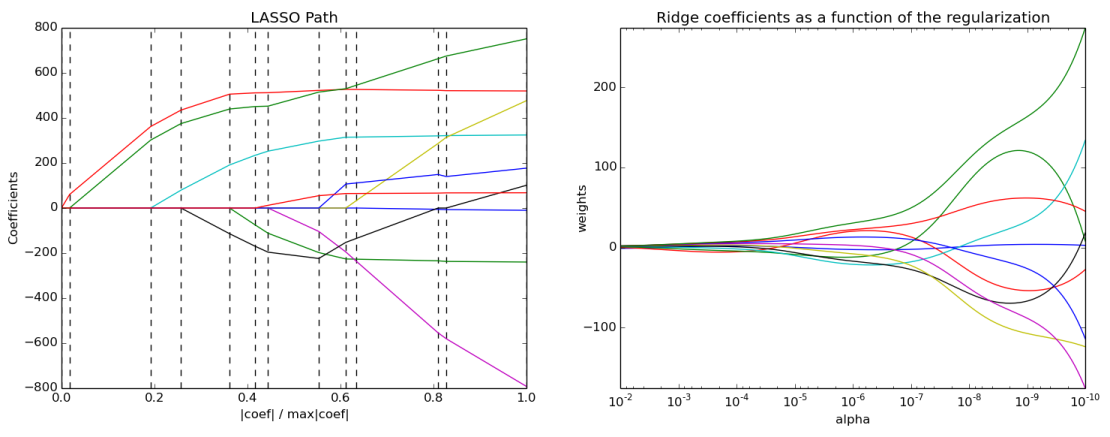
\includegraphics{./assets/lasso_ridge_path.png}
\caption{Lasso and Ridge Coefficient Plots}
\end{figure}

     \#\#\# Advice for Applying Regularization

\textbf{Should features be standardized?}

\begin{itemize}
\tightlist
\item
  Yes, because otherwise, features would be penalized simply because of
  their scale.
\item
  Also, standardizing avoids penalizing the intercept, which wouldn't
  make intuitive sense.
\end{itemize}

\textbf{How should you choose between lasso regression and ridge
regression?}

\begin{itemize}
\tightlist
\item
  Lasso regression is preferred if we believe many features are
  irrelevant or if we prefer a sparse model.
\item
  Ridge can work particularly well if there is a high degree of
  multicollinearity in your model.
\item
  If model performance is your primary concern, it is best to try both.
\item
  Elastic net regression is a combination of lasso regression and ridge
  Regression.
\end{itemize}

     \#\#\# Ridge Regression

\begin{itemize}
\tightlist
\item
  \href{http://scikit-learn.org/stable/modules/generated/sklearn.linear_model.Ridge.html}{Ridge}
  documentation
\item
  \textbf{alpha:} must be positive, increase for more regularization
\item
  \textbf{normalize:} scales the features (without using StandardScaler)
\end{itemize}

    \begin{Verbatim}[commandchars=\\\{\}]
{\color{incolor}In [{\color{incolor}83}]:} \PY{c+c1}{\PYZsh{} Include dummy variables for season in the model.}
         \PY{n}{feature\PYZus{}cols} \PY{o}{=} \PY{p}{[}\PY{l+s+s1}{\PYZsq{}}\PY{l+s+s1}{temp}\PY{l+s+s1}{\PYZsq{}}\PY{p}{,} \PY{l+s+s1}{\PYZsq{}}\PY{l+s+s1}{atemp}\PY{l+s+s1}{\PYZsq{}}\PY{p}{,} \PY{l+s+s1}{\PYZsq{}}\PY{l+s+s1}{season\PYZus{}2}\PY{l+s+s1}{\PYZsq{}}\PY{p}{,} \PY{l+s+s1}{\PYZsq{}}\PY{l+s+s1}{season\PYZus{}3}\PY{l+s+s1}{\PYZsq{}}\PY{p}{,} \PY{l+s+s1}{\PYZsq{}}\PY{l+s+s1}{season\PYZus{}4}\PY{l+s+s1}{\PYZsq{}}\PY{p}{,} \PY{l+s+s1}{\PYZsq{}}\PY{l+s+s1}{humidity}\PY{l+s+s1}{\PYZsq{}}\PY{p}{]}
         
         \PY{n}{X} \PY{o}{=} \PY{n}{bikes\PYZus{}dummies}\PY{p}{[}\PY{n}{feature\PYZus{}cols}\PY{p}{]}
         \PY{n}{y} \PY{o}{=} \PY{n}{bikes\PYZus{}dummies}\PY{o}{.}\PY{n}{total\PYZus{}rentals}
\end{Verbatim}


    \begin{Verbatim}[commandchars=\\\{\}]
{\color{incolor}In [{\color{incolor}84}]:} \PY{n}{X\PYZus{}train}\PY{p}{,} \PY{n}{X\PYZus{}test}\PY{p}{,} \PY{n}{y\PYZus{}train}\PY{p}{,} \PY{n}{y\PYZus{}test} \PY{o}{=} \PY{n}{train\PYZus{}test\PYZus{}split}\PY{p}{(}\PY{n}{X}\PY{p}{,} \PY{n}{y}\PY{p}{,} \PY{n}{random\PYZus{}state}\PY{o}{=}\PY{l+m+mi}{1}\PY{p}{)}
\end{Verbatim}


    \begin{Verbatim}[commandchars=\\\{\}]
{\color{incolor}In [{\color{incolor}85}]:} \PY{c+c1}{\PYZsh{} alpha=0 is equivalent to linear regression.}
         \PY{k+kn}{from} \PY{n+nn}{sklearn}\PY{n+nn}{.}\PY{n+nn}{linear\PYZus{}model} \PY{k}{import} \PY{n}{Ridge}\PY{p}{,} \PY{n}{Lasso}
         
         \PY{c+c1}{\PYZsh{} Instantiate the model.}
         \PY{c+c1}{\PYZsh{}(Alpha of zero has no regularization strength, essentially a basic linear regression.)}
         \PY{n}{ridgereg} \PY{o}{=} \PY{n}{Ridge}\PY{p}{(}\PY{n}{alpha}\PY{o}{=}\PY{l+m+mi}{0}\PY{p}{,} \PY{n}{normalize}\PY{o}{=}\PY{k+kc}{True}\PY{p}{)}
         
         \PY{c+c1}{\PYZsh{} Fit the model.}
         \PY{n}{ridgereg}\PY{o}{.}\PY{n}{fit}\PY{p}{(}\PY{n}{X\PYZus{}train}\PY{p}{,} \PY{n}{y\PYZus{}train}\PY{p}{)}
         
         \PY{c+c1}{\PYZsh{} Predict with fitted model.}
         \PY{n}{y\PYZus{}pred} \PY{o}{=} \PY{n}{ridgereg}\PY{o}{.}\PY{n}{predict}\PY{p}{(}\PY{n}{X\PYZus{}test}\PY{p}{)}
         \PY{n+nb}{print}\PY{p}{(}\PY{n}{np}\PY{o}{.}\PY{n}{sqrt}\PY{p}{(}\PY{n}{metrics}\PY{o}{.}\PY{n}{mean\PYZus{}squared\PYZus{}error}\PY{p}{(}\PY{n}{y\PYZus{}test}\PY{p}{,} \PY{n}{y\PYZus{}pred}\PY{p}{)}\PY{p}{)}\PY{p}{)}
\end{Verbatim}


    \begin{Verbatim}[commandchars=\\\{\}]
156.67429349903927

    \end{Verbatim}

    \begin{Verbatim}[commandchars=\\\{\}]
{\color{incolor}In [{\color{incolor}86}]:} \PY{c+c1}{\PYZsh{} Coefficients for a non\PYZhy{}regularized linear regression}
         \PY{n+nb}{list}\PY{p}{(}\PY{n+nb}{zip}\PY{p}{(}\PY{n}{feature\PYZus{}cols}\PY{p}{,} \PY{n}{ridgereg}\PY{o}{.}\PY{n}{coef\PYZus{}}\PY{p}{)}\PY{p}{)}
\end{Verbatim}


\begin{Verbatim}[commandchars=\\\{\}]
{\color{outcolor}Out[{\color{outcolor}86}]:} [('temp', 8.537530902593584),
          ('atemp', 2.4548540987561642),
          ('season\_2', -9.325429567785928),
          ('season\_3', -40.6789961974648),
          ('season\_4', 61.11748928364946),
          ('humidity', -2.865044830544153)]
\end{Verbatim}
            
    To interpret these coefficients we need to convert them back to original
units, which is a reason to do normalization by hand. However, in this
form the coefficients have a special meaning. The intercept is now the
average of our outcome, and the magnitude of each coefficient in the
model is a measure of how important it is in the model. We call this
feature importance.

    \begin{Verbatim}[commandchars=\\\{\}]
{\color{incolor}In [{\color{incolor}87}]:} \PY{c+c1}{\PYZsh{} Try alpha=0.1.}
         \PY{n}{ridgereg} \PY{o}{=} \PY{n}{Ridge}\PY{p}{(}\PY{n}{alpha}\PY{o}{=}\PY{l+m+mf}{0.1}\PY{p}{,} \PY{n}{normalize}\PY{o}{=}\PY{k+kc}{True}\PY{p}{)}
         \PY{n}{ridgereg}\PY{o}{.}\PY{n}{fit}\PY{p}{(}\PY{n}{X\PYZus{}train}\PY{p}{,} \PY{n}{y\PYZus{}train}\PY{p}{)}
         \PY{n}{y\PYZus{}pred} \PY{o}{=} \PY{n}{ridgereg}\PY{o}{.}\PY{n}{predict}\PY{p}{(}\PY{n}{X\PYZus{}test}\PY{p}{)}
         \PY{n+nb}{print}\PY{p}{(}\PY{n}{np}\PY{o}{.}\PY{n}{sqrt}\PY{p}{(}\PY{n}{metrics}\PY{o}{.}\PY{n}{mean\PYZus{}squared\PYZus{}error}\PY{p}{(}\PY{n}{y\PYZus{}test}\PY{p}{,} \PY{n}{y\PYZus{}pred}\PY{p}{)}\PY{p}{)}\PY{p}{)}
\end{Verbatim}


    \begin{Verbatim}[commandchars=\\\{\}]
156.96098662565277

    \end{Verbatim}

    \begin{Verbatim}[commandchars=\\\{\}]
{\color{incolor}In [{\color{incolor}88}]:} \PY{c+c1}{\PYZsh{} Examine the coefficients.}
         \PY{n+nb}{list}\PY{p}{(}\PY{n+nb}{zip}\PY{p}{(}\PY{n}{feature\PYZus{}cols}\PY{p}{,} \PY{n}{ridgereg}\PY{o}{.}\PY{n}{coef\PYZus{}}\PY{p}{)}\PY{p}{)}
\end{Verbatim}


\begin{Verbatim}[commandchars=\\\{\}]
{\color{outcolor}Out[{\color{outcolor}88}]:} [('temp', 5.257452659873023),
          ('atemp', 4.254523291538834),
          ('season\_2', -0.17934556275242566),
          ('season\_3', -21.48394260544527),
          ('season\_4', 56.6822078418667),
          ('humidity', -2.658837791464091)]
\end{Verbatim}
            
    While the MSE barely improved, we can see there are significant changes
in the weight of our coefficients. Particularly \texttt{season\_2} whose
coefficient has greatly decreased toward 0.

Fitting and using a Lasso Regression in scikit-learn is very similar.

In addition to the typical
\href{http://scikit-learn.org/stable/modules/generated/sklearn.linear_model.Lasso.html}{lasso}
and
\href{http://scikit-learn.org/stable/modules/generated/sklearn.linear_model.Ridge.html}{ridge}
there is a third type of regression,
\href{http://scikit-learn.org/stable/modules/generated/sklearn.linear_model.ElasticNet.html}{Elastic
Net} which combines the penalties of the ridge and lasso methods.

     \#\# Comparing Linear Regression With Other Models

Advantages of linear regression:

\begin{itemize}
\tightlist
\item
  Simple to explain.
\item
  Highly interpretable.
\item
  Model training and prediction are fast.
\item
  No tuning is required (excluding regularization).
\item
  Features don't need scaling.
\item
  Can perform well with a small number of observations.
\item
  Well understood.
\end{itemize}

Disadvantages of linear regression:

\begin{itemize}
\tightlist
\item
  Presumes a linear relationship between the features and the response.
\item
  Performance is (generally) not competitive with the best supervised
  learning methods due to high bias.
\item
  Can't automatically learn feature interactions.
\end{itemize}


    % Add a bibliography block to the postdoc
    
    
    
    \end{document}
